\newtheorem{theorem}{Theorem}
\newtheorem{lemma}{Lemma}
\newtheorem{corollary}{Corollary}
\newtheorem{proposition}{Proposition}

% This is paper.tex

\section{Introduction}
A planar graph is a graph that can be embedded into the plane, meaning that one can draw the graph on a plane in such a way that its edges do not cross each other. In other words, its edges only intersect at the edges' endpoints. Common examples of planar graphs are $K_3$ and $K_4$, shown in figure \ref{k3k4}.

\begin{figure}[h]
	\centering
	\begin{tabular}{c|c}
		\hline
		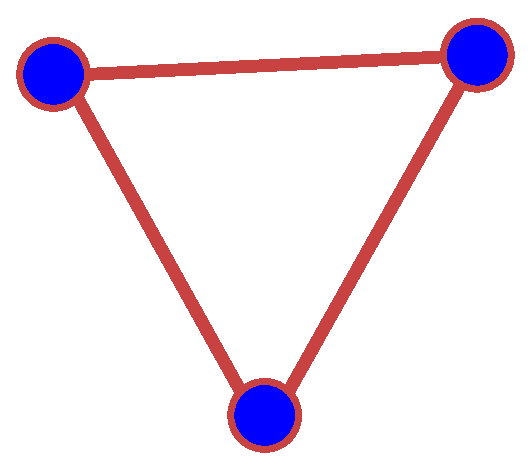
\includegraphics[height=1.5in]{k3.eps} & 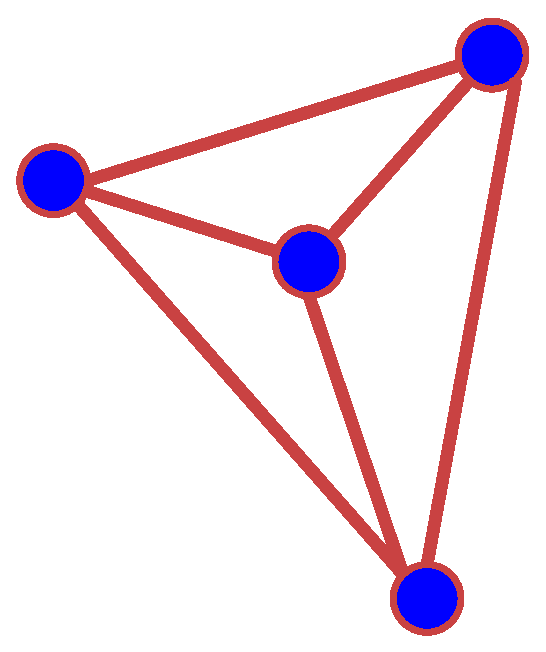
\includegraphics[height=1.5in]{k4.eps} \\ 
		\textbf{$K_3$} & \textbf{$K_4$} \\
		\hline
	\end{tabular}
		\caption{Planar graphs $K_3$ and $K_4$.}
\label{k3k4}
\end{figure}

Planar graphs can be used to model a variety of real-life systems. For example, in the field of vehicle routing, planar graphs can be used to represent routes on highway systems without any overpasses or underpasses. Another application is in very-large-scale integration (VLSI), which involves the design of integrated circuits on a single chip.  On the chip, transistors are laid out such that none of them intersect with each other.

In this paper, we explore the conditions under which a graph is considered planar. We discuss and prove Kuratowski's Theorem, which states that a graph is planar if and only if it does not contain a minor of either the graph $K_{3,3}$ or the graph $K_5$.

\section{Prerequisite Definitions}  
In this section we recall some definitions of graph theory. A \emph{graph G} is a pair (V,E) of finite sets, where $V$ is the set of all vertices in the graph and $E$ is the set of all edges in the graph. An edge, (an element in the set E) connects an element $v_i$ in the set V either with itself $(v_i,v_i)$ or with another vertex $v_k$ in the set V. The \emph{degree} of a vertex $v$ of a graph is the number of edges connected to the vertex. The \emph{maximum degree} of a graph $G$, denoted $\Delta(G)$, is the value of the maximum degree of any given vertex in the graph. Figure \ref{degree} shows a graph with each of the vertices labeled with its degree. The maximum degree of the graph is the highest degree of the graph's vertices, $\Delta(G) = 3$. 
\begin{figure}[htbp]
	\centering
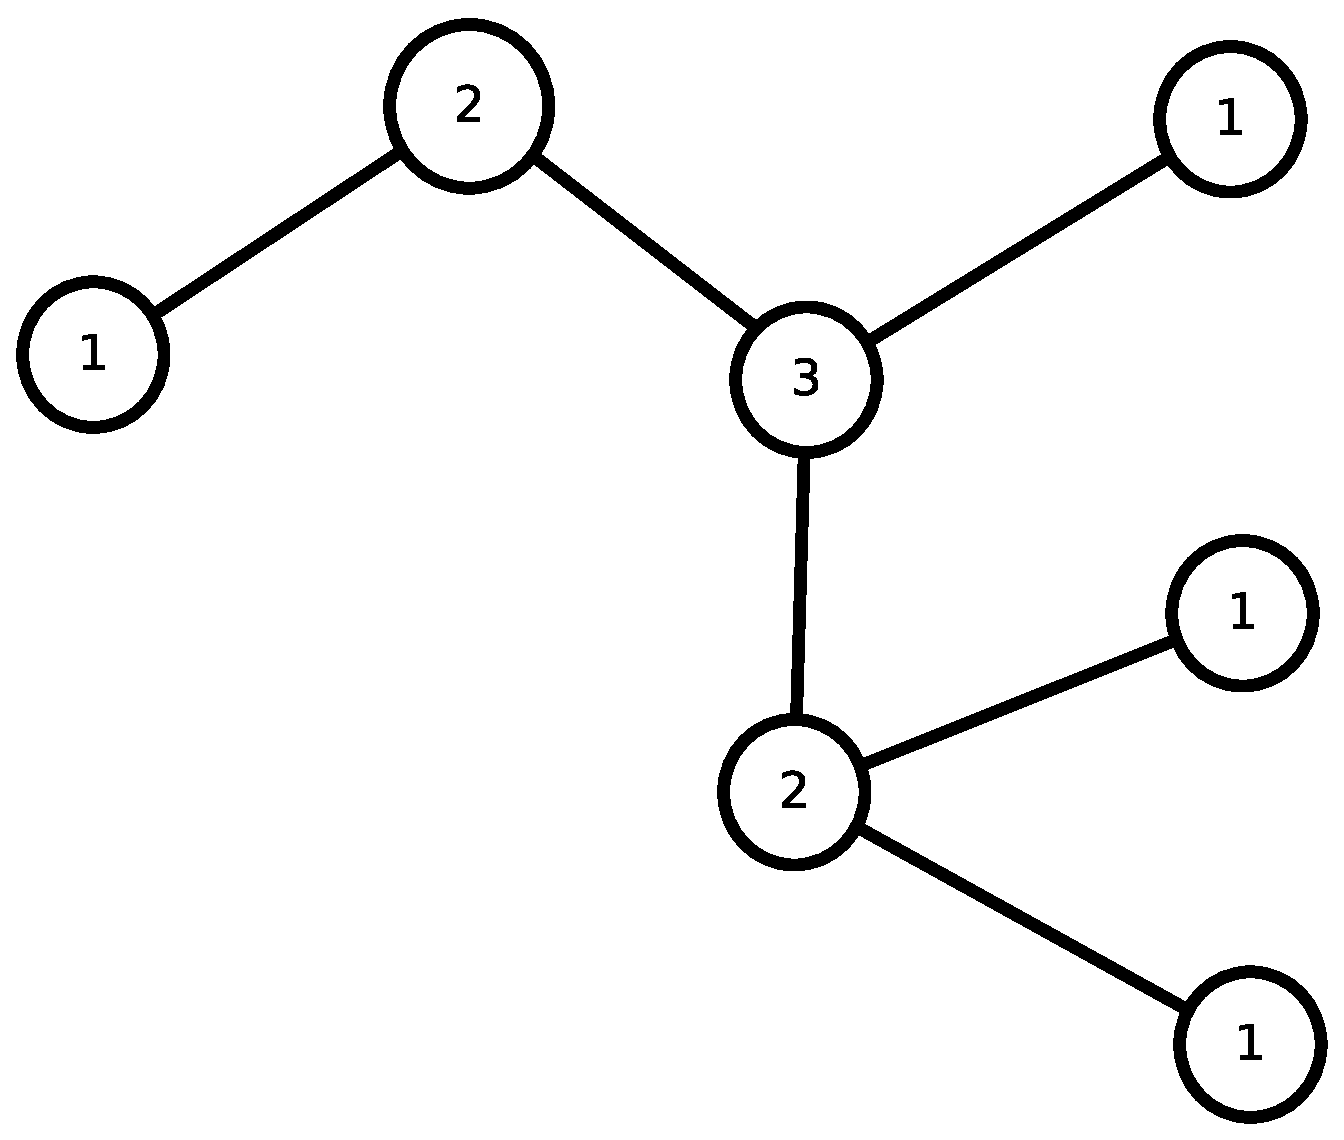
\includegraphics[height=1.5in]{degree.eps}
\caption{A graph $G$ with each of its vertices labeled with its degree. The maximum degree is $\Delta(G) = 3$.}
\label{degree}
\end{figure}

In a graph, a \emph{path} from vertex $v_1$ to $v_n$ is a sequence of edges where the first edge contains $v_1$, the last edge contains $v_n$, and a common vertex connects a pair of two edges for all edges that lie between $v_1$ and $v_n$. For example in figure \ref{fig1}, the path $\{(a,b), (b,c),(c,d)\}$ connects the vertices $a$ and $b$. 
\begin{figure}[htbp]
	\centering
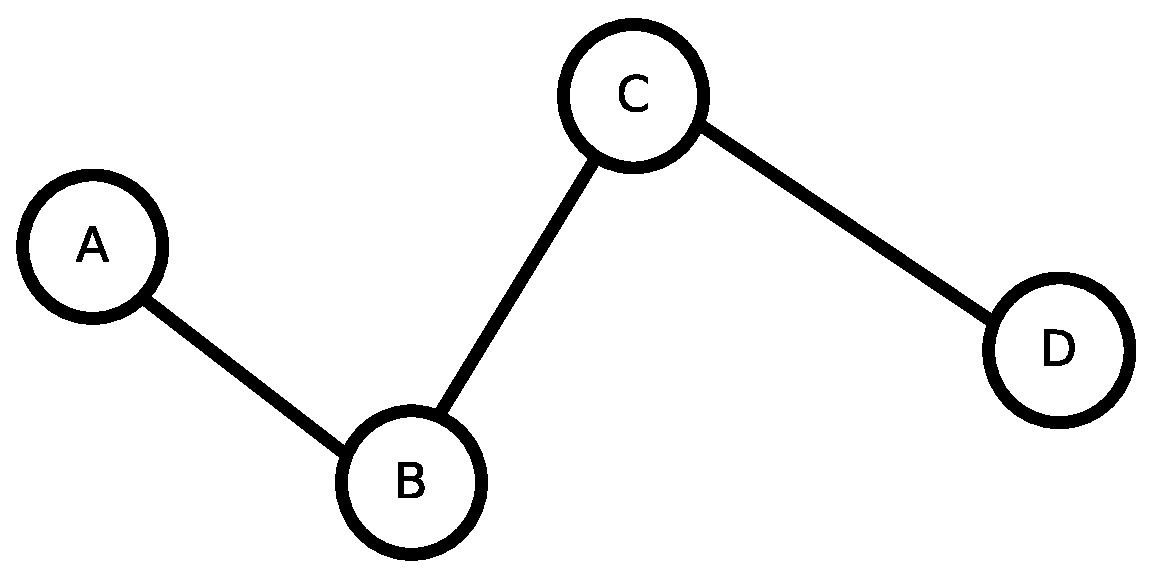
\includegraphics[height=1.5in]{path.eps}
\caption{A path.}
\label{fig1}
\end{figure}
A \emph{cycle} is a path such that the start vertex and end vertex are the same. For example, in figure \ref{cycle}, the path $\{(a,b),(b,c),(c,d),(d,e),(e,a)\}$ is a cycle. 
\begin{figure}[htbp]
	\centering
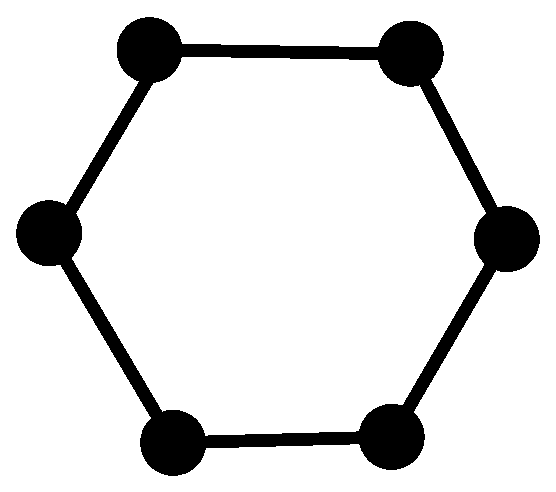
\includegraphics[height=1.5in]{cycle.eps}
\caption{A cycle.}
\label{cycle}
\end{figure}
Given a cycle,a \emph{chord} is an edge that connects two vertices on a cycle which are not adjacent. For example, in the graph in figure \ref{chord}, a chord connects non-adjacent vertices $a$ and $b$ in the graph.
\begin{figure}
	\centering
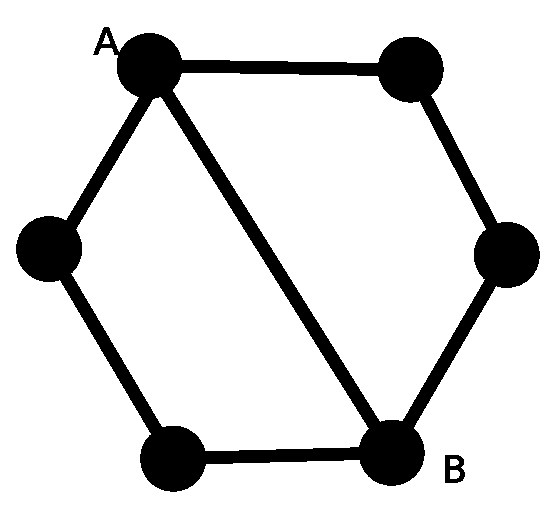
\includegraphics[height=1.5in]{chord.eps}
\caption{A chord connecting vertex $a$ and vertex $b$.}
\label{chord}
\end{figure}
A \emph{connected graph} is a graph such that for any two vertices in V, there is a path from one vertex to the other. The graphs in figure \ref{cycle} and figure \ref{chord} are connected.

A \emph{subgraph} of the graph G is a graph H with a set of vertices that is contained in V and a set of edges that is contained in E.  A \emph{partition} of a graph G is defined as a partition of E and V into the subsets $V_k$ and $E_k$ such that the edges in $E_k$ have endpoints in $V_k$. We can partition a graph into maximal connected subgraphs. The maximal connected subgraphs are subgraphs such that there is no path that connects a vertex from one subgraph to another. If a graph is not connected then you can partition it into subgraphs, each of which are indeed connected. The graph in figure \ref{4comp} has 4 separate maximal connected components.
	
\begin{figure}
	\centering
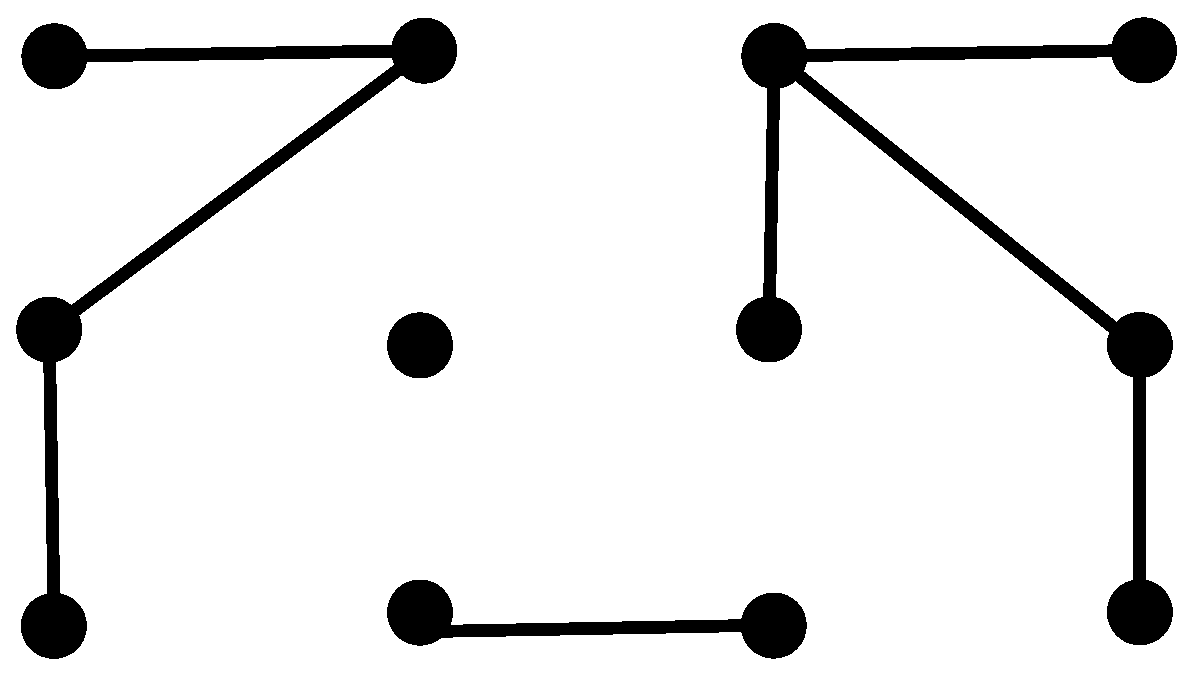
\includegraphics[height=1.5in]{4comp.eps}
\caption{A graph with 4 connected components.}
\label{4comp}
\end{figure}

A \emph{bridge} is an edge which, when deleted, increases the number of connected components in the graph. For example, in the graph in figure \ref{bridge}, when the bridge (a,b) is deleted, the number of connected components in the graph increases from 4 to 5.

\begin{figure}
	\centering
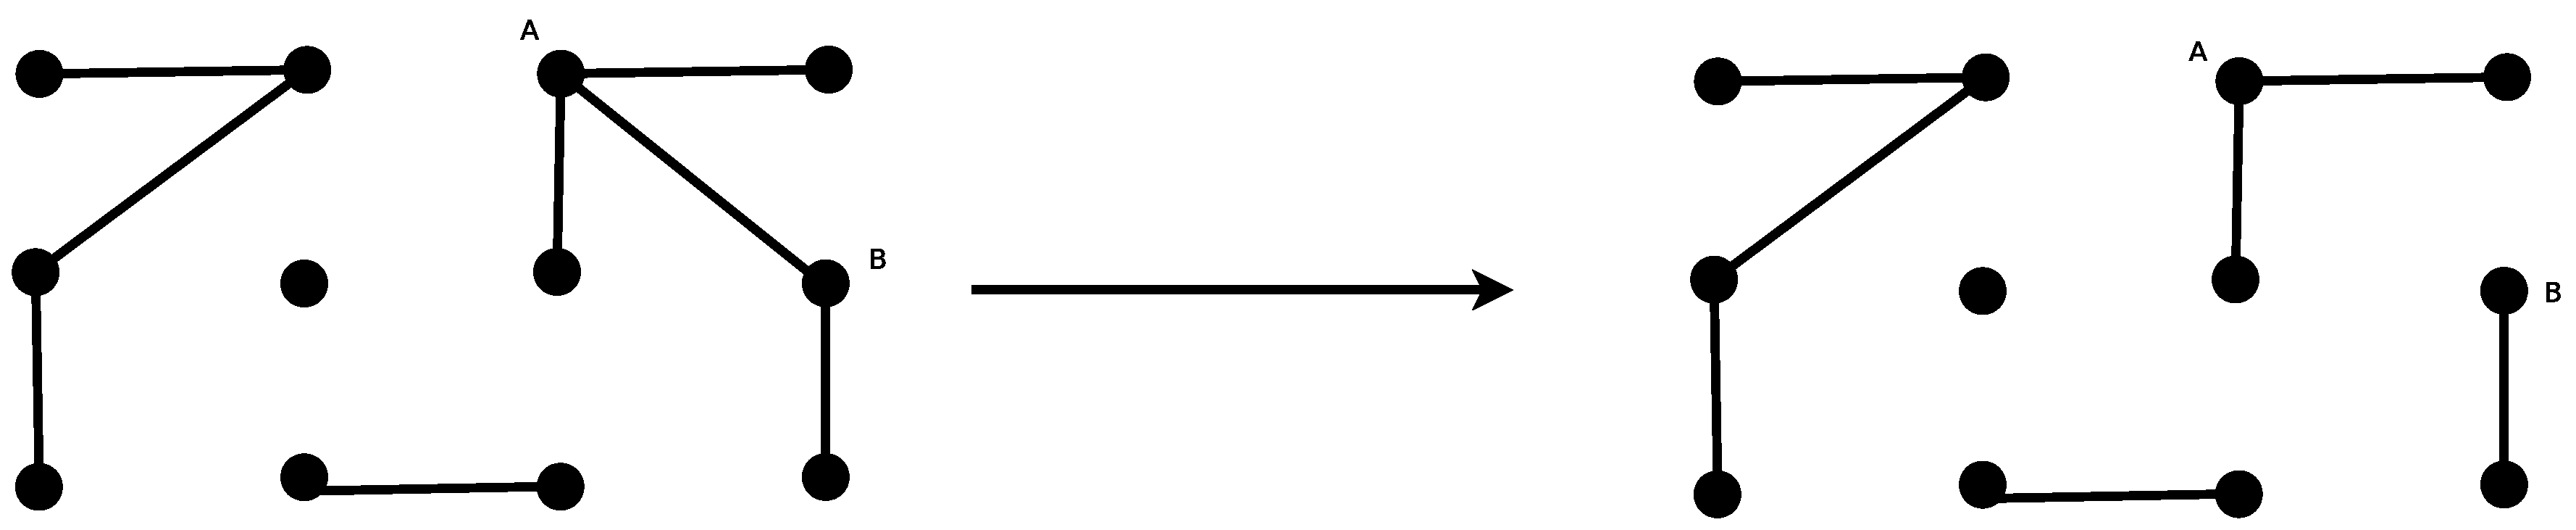
\includegraphics[height=1.2in]{bridge.eps}
\caption{A bridge $(a,b)$.}
\label{bridge}
\end{figure}

A \emph{complete graph} is a graph where every pair of vertices is connected by a unique edge. Formally, we define a complete graph $K_n$ to be a graph with n vertices such that every possible edge is contained in the set of edges. 	
A \emph{bipartite graph} is a graph that can be partitioned into two subsets such that no two vertices that are connected by a shared edge are contained in the same subset. We denote $K_{m,n}$ to be a complete, bipartite graph containing two partitions of vertices of sizes $m$ and $n$. An example would be $K_{3,2}$ which is shown in figure \ref{fig2}.  Notice that there are two subsets of vertices, one subset of two vertices on the left side and one subset of three vertices on the right side. Every edge connects a vertex from one subset to  a vertex in the other subset.

\begin{figure}
	\centering
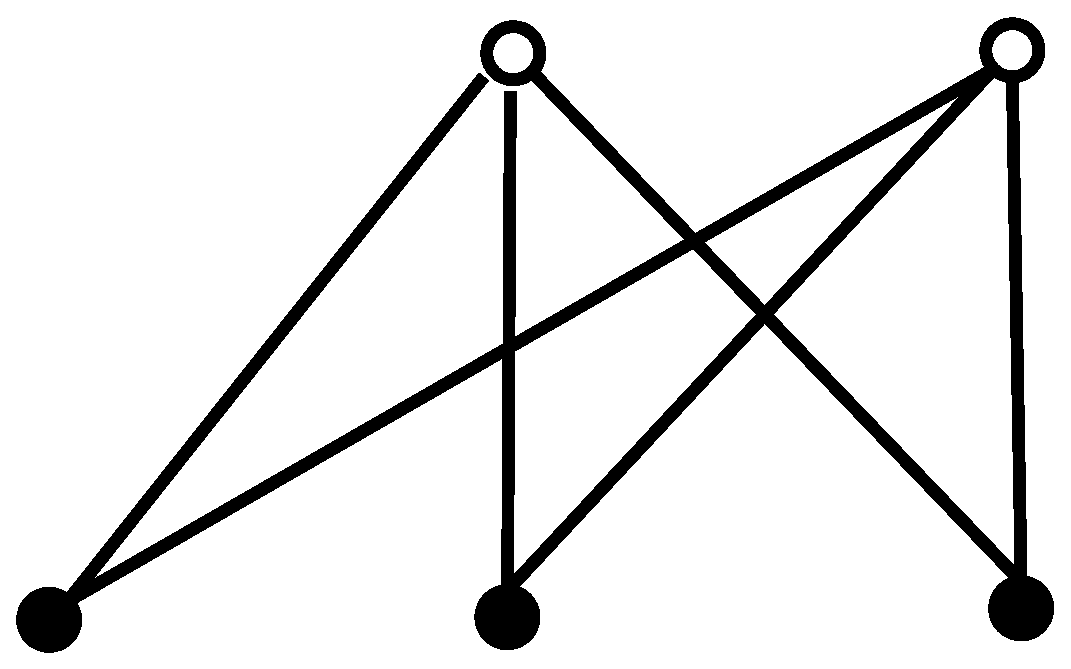
\includegraphics[height=1.5in]{fig2.eps}
\caption{Bipartite graph.}
\label{fig2}
\end{figure}

\begin{figure}
	\centering
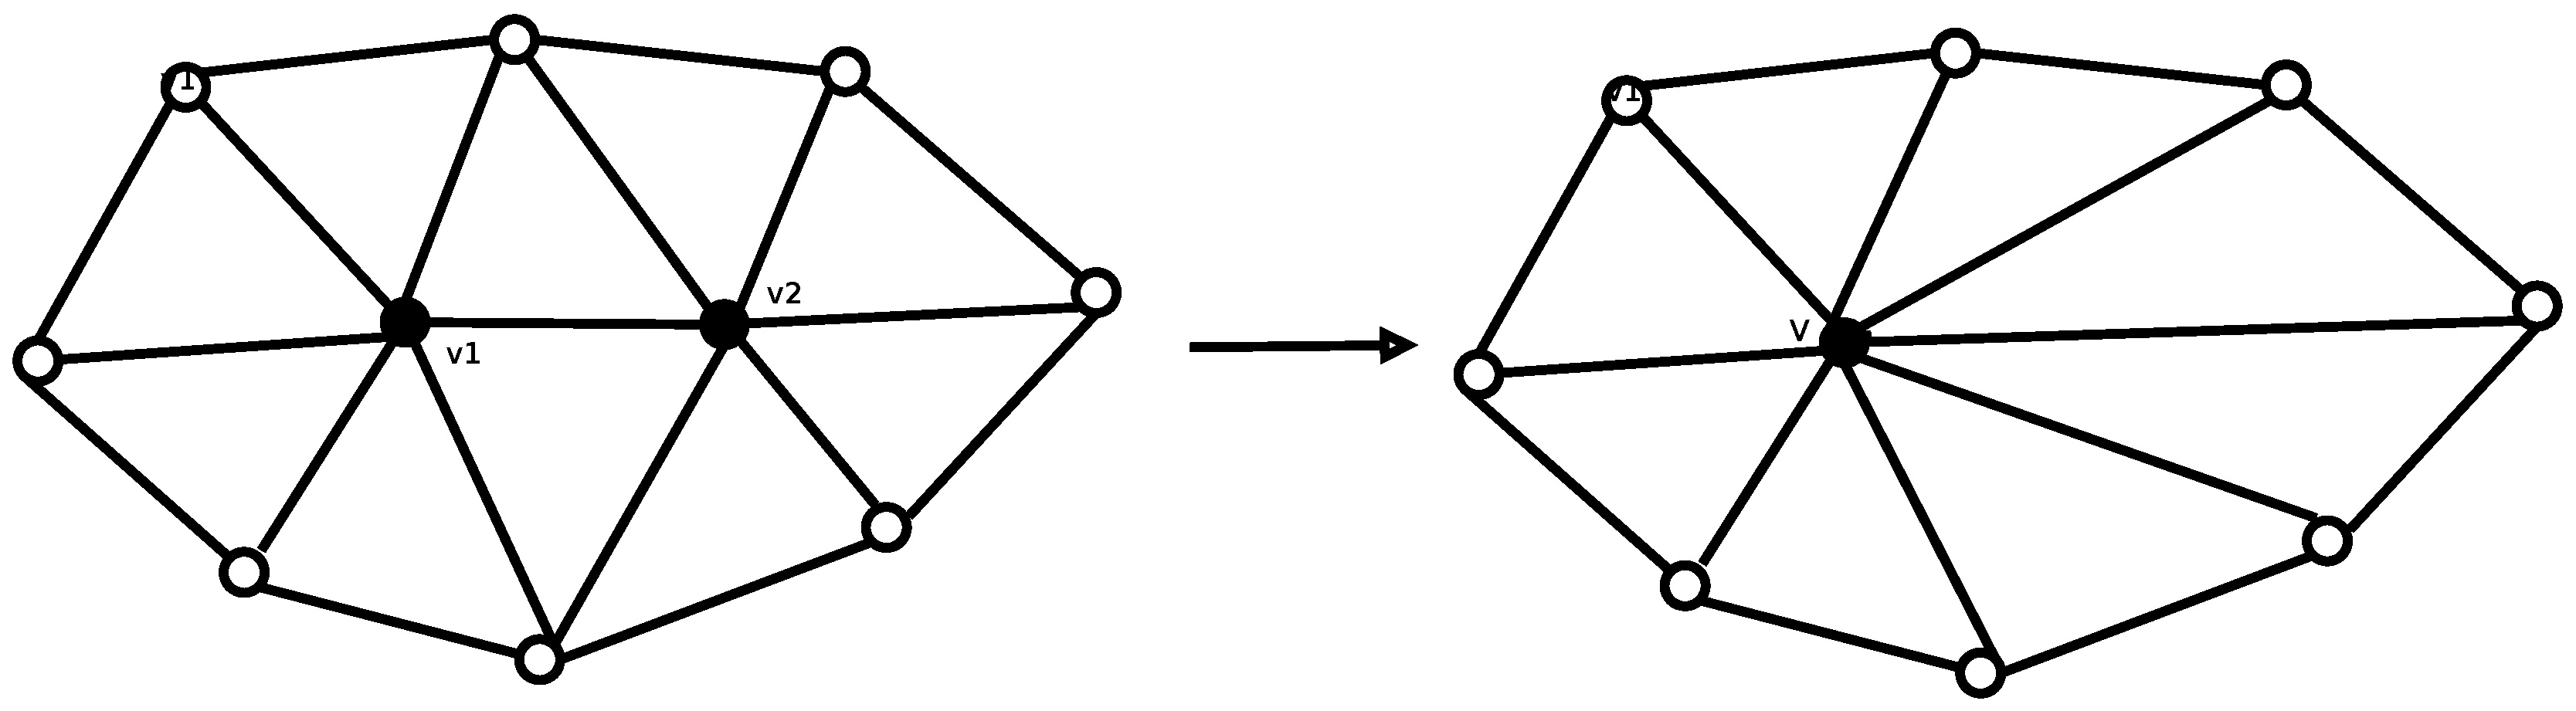
\includegraphics[height=1.5in]{contract.eps}
\caption{Contraction of the edge $(v_1, v_2)$ results in a graph with a new vertex $\bar{v}$.}
\label{contract}
\end{figure} 

An \emph{edge contraction} is an operation which removes an edge from a graph and merges the two vertices that the edge connected into one single vertex. An example is shown in figure \ref{contract}, where the edge $(v_1, v_2)$ is contracted to a vertex $\bar{v}$. A graph H is called a \emph{minor} of the graph G, if H is isomorphic to a graph that can be obtained by zero or more edge contractions on a subgraph of G. A \emph{subdivision} of a graph $G$ is a graph resulting from the subdivision of edges in $G$. The subdivision of an edge $e$ with endpoints $(u,v)$ yields a graph that contains a new vertex $w$, such that the edge $e$ is replaced by two new edges $(u,w)$ and $(w,v)$ (See figure \ref{subdivision}). An isomorphism of graph $G$ and $H$ is a bijection between the vertex sets of $G$ and $H$:
$$f:V(G) \rightarrow V(H)$$
such that two vertices $u$ and $v$ are adjacent in $G$ if and only if $f(u)$ and $f(v)$ are adjacent in $H$. Two graphs are \emph{isomorphic} if an isomorphism exists between the two graphs. 

\begin{figure}
	\centering
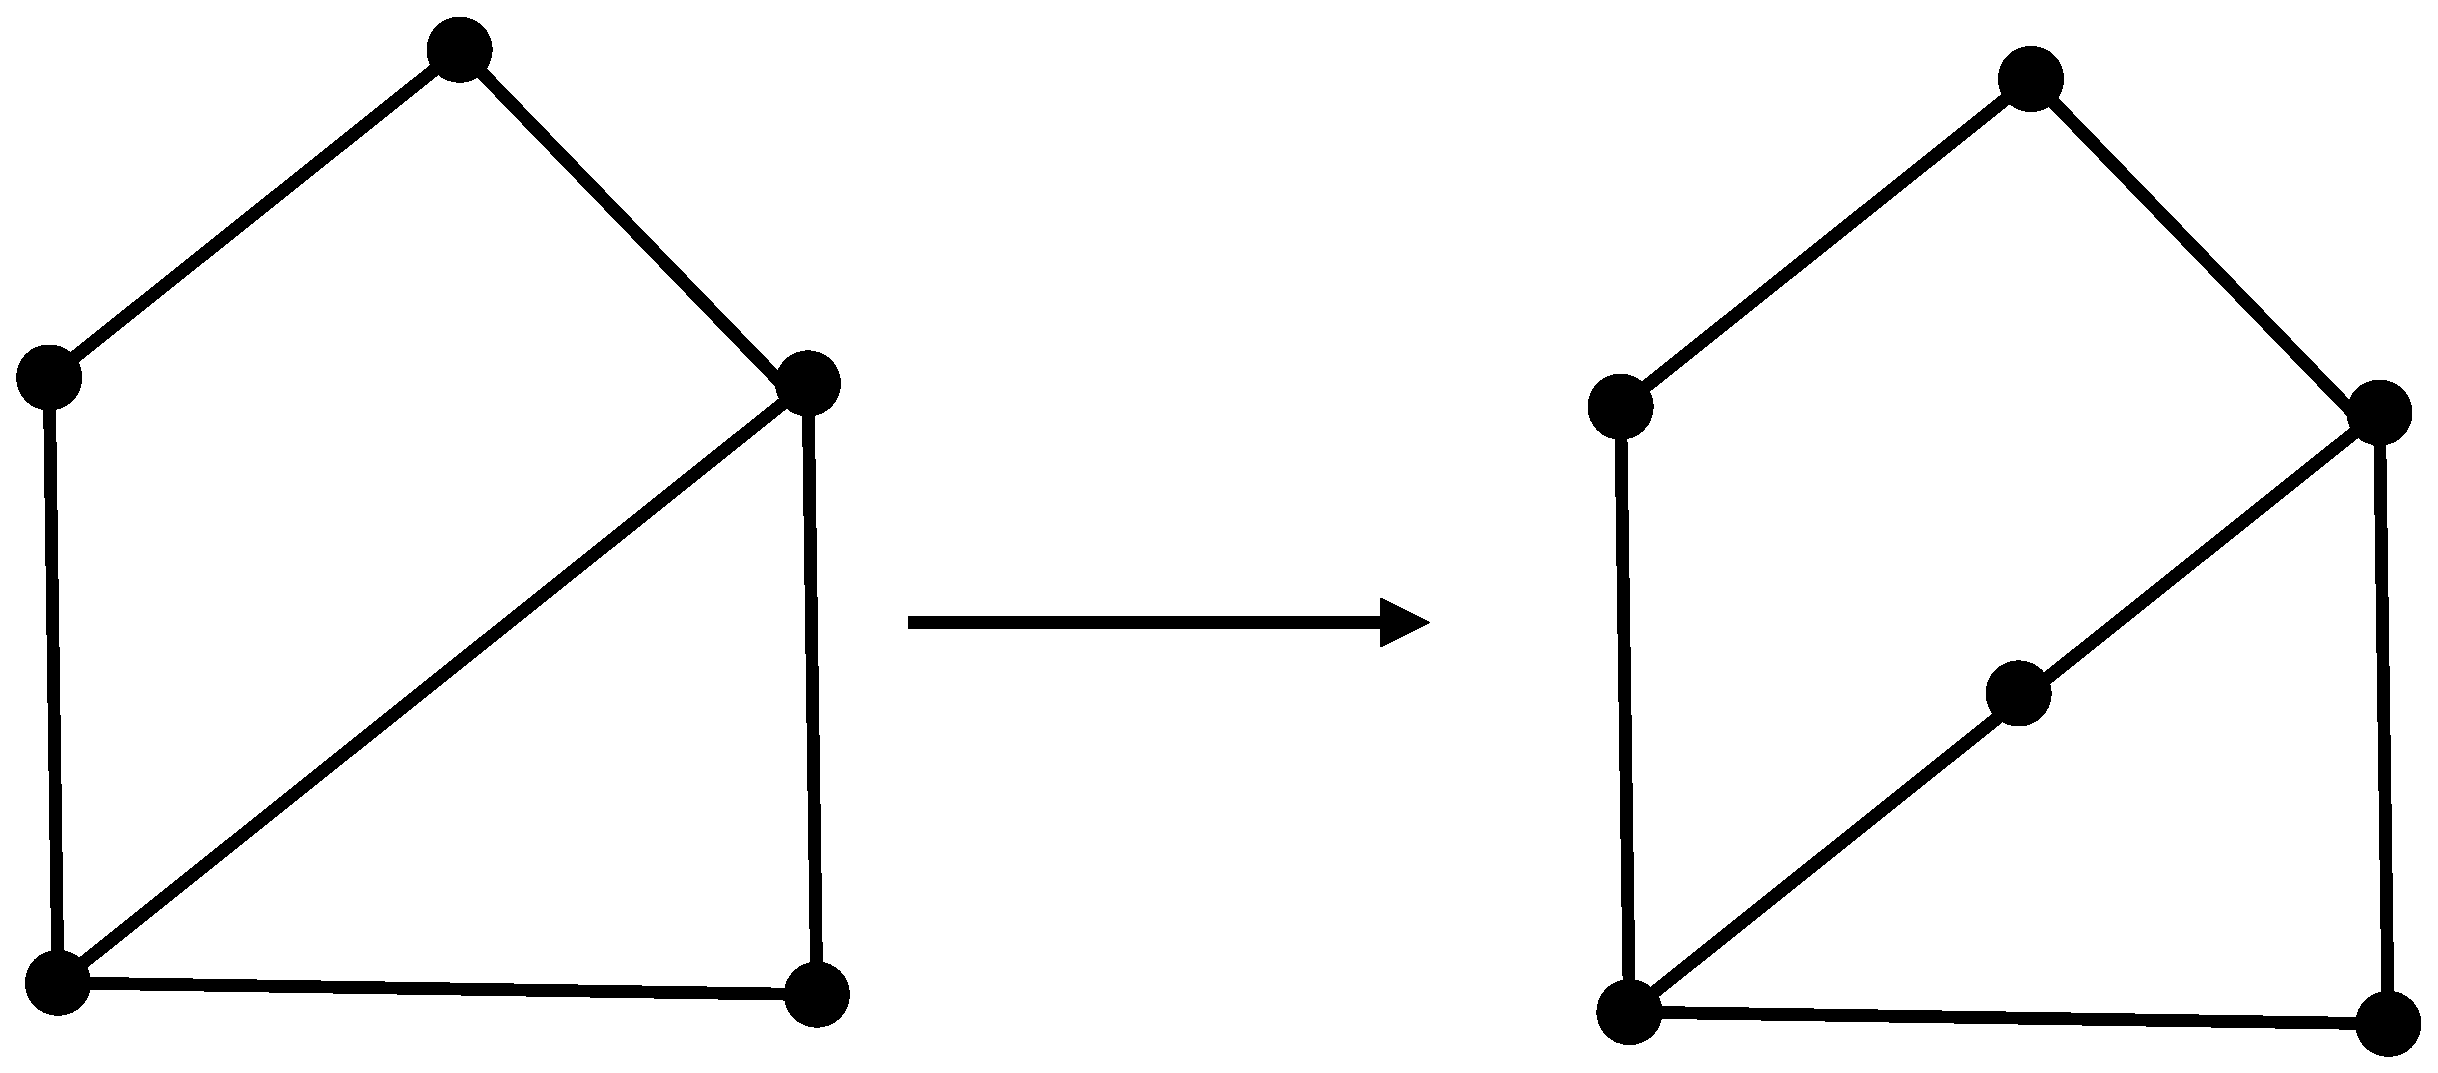
\includegraphics[height=1.5in]{subdivision.eps}
\caption{A subdivision of the edge $(u,v)$ yields two new edges $(u,w)$ and $(w,v)$.}
\label{subdivision}
\end{figure} 

\begin{figure}
	\centering
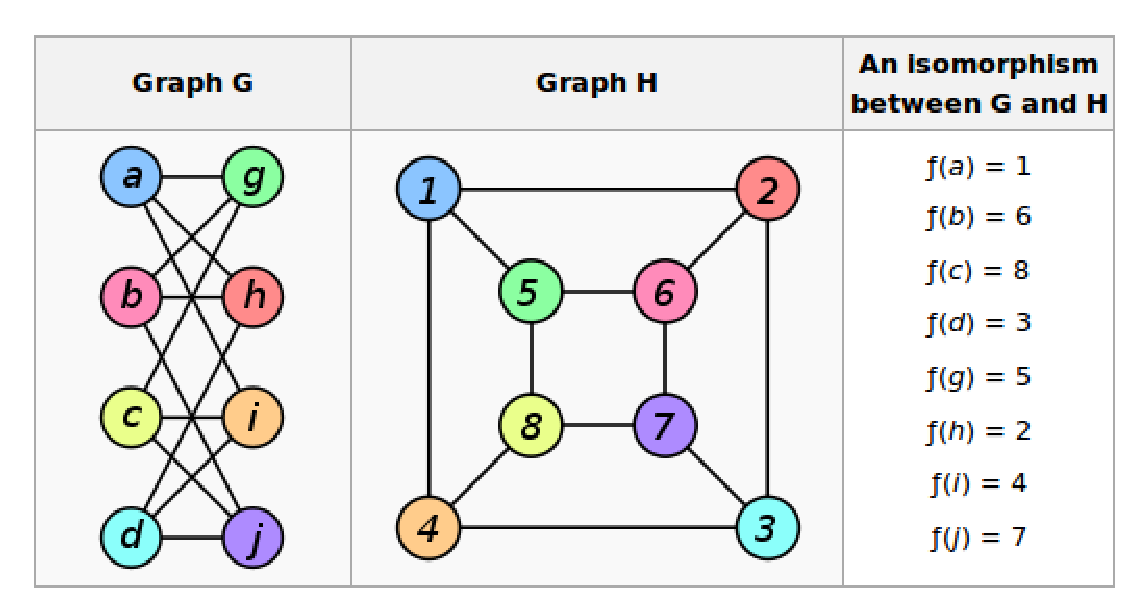
\includegraphics[height=1.5in]{isomorphism.eps}
\caption{An isomorphism.}
\label{isomorphism}
\end{figure}
%%%%%%%%%%%%%%%%%%%%%%%%%%%%%%%%%%%%%%%%%%%%%%%%%%%%%%%%%
\subsection{Planar Graphs}
A \emph{planar graph} is a graph that can be embedded in the plane.  That is, it can be drawn on a plane in such a way that its edges do not cross each other. In other words, its edges only intersect at the edges' endpoints. A planar graph that is drawn in the plane without edge crossings is a \emph{plane graph}. Note that a planar graph can be drawn in a plane \emph{with} edge crossings, in which case it would \emph{not} be considered a plane graph. The graph $K_4$, shown in figure \ref{k4_plane}, demonstrates this. A \emph{planar drawing} of a planar graph is a drawing of the graph in the plane such that no edge crossings occur. Figure \ref{k4_plane}B shows a planar drawing of the $K_4$ graph. A \emph{non-planar drawing} of a planar graph is a drawing of the graph in the plane such that there is at least one edge crossing. Figure \ref{k4_plane}A shows a non-planar drawing of the $K_4$ graph.
%%%%%%%%%%%%%%%%%%%%%%%%%%%%
\begin{figure}[h]
	\centering
	\begin{tabular}{c|c}
		\hline
		A & B\\
		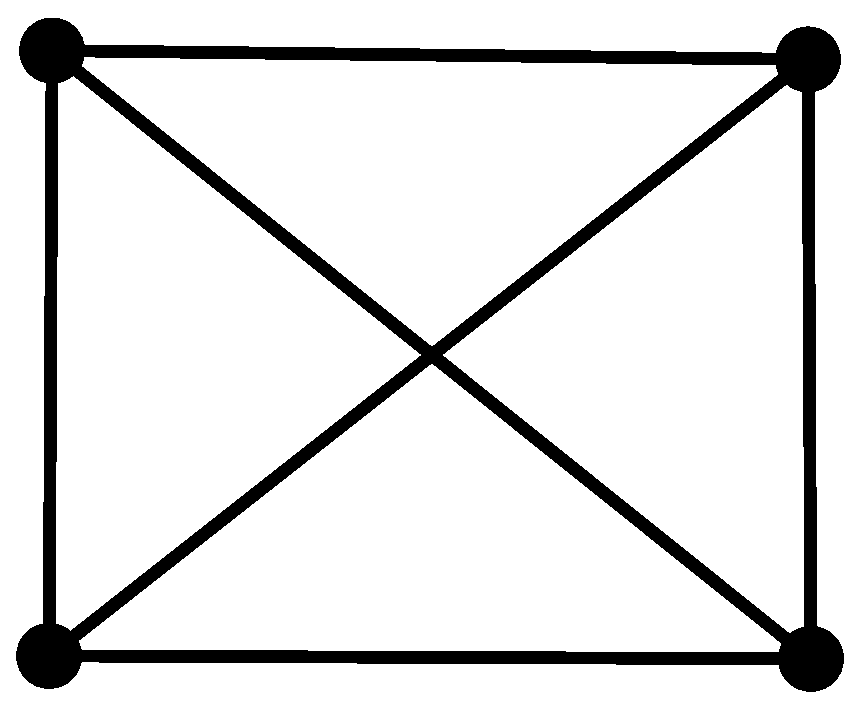
\includegraphics[height=1.5in]{k4_cross.eps} & 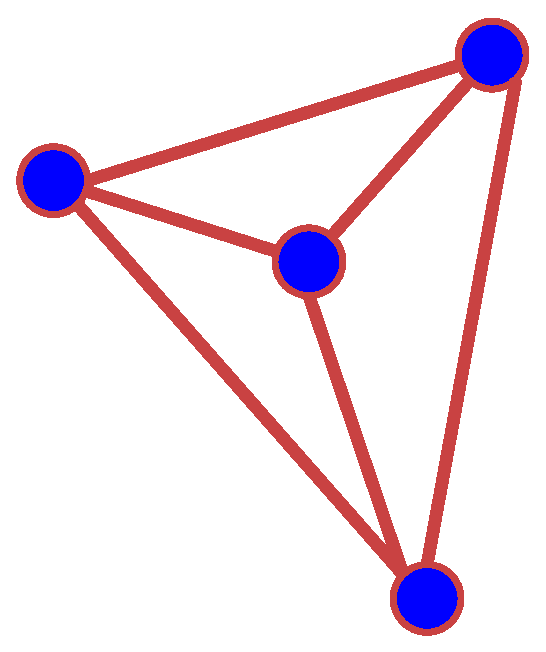
\includegraphics[height=1.5in]{k4.eps} \\ 
		\textbf{$K_4$, not a plane graph} & \textbf{plane graph of $K_4$} \\
		\hline
	\end{tabular}
	\caption{(A) The graph  $K_4$ is a planar graph, but here it is not drawn as a plane graph because two edges intersect. (B) The graph of $K_4$ drawn as a plane graph, as it is embedded in the plane without edge crossings.}
\label{k4_plane}
\end{figure}
%%%%%%%%%%%%%%%%%%%%%%%%%%%%%%%%%%%%%%%%%%%%%%%%%%%%%%%%%%%%%%%%%%%%%%%%%%%%%%%%%%%%%%%%%%%%%%%%%%%%%%%%%
A \emph{maximally planar graph} is a planar graph that cannot have edges added to it while violating the planarity of G. An example of maximally planar graph is $K_3$ (see Figure \ref{fig3}).

\begin{figure}
	\centering
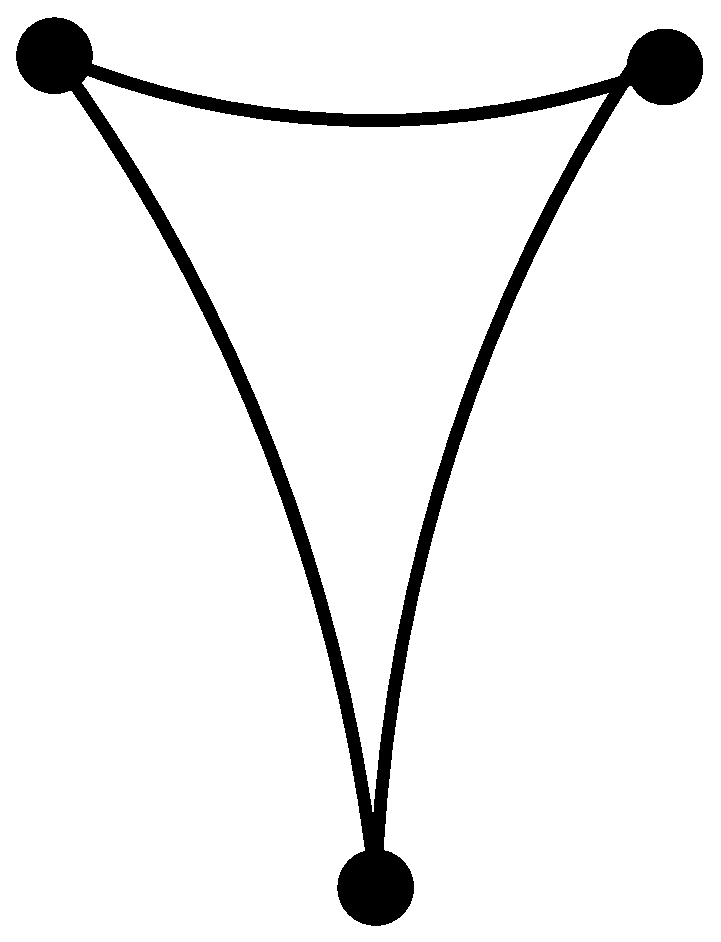
\includegraphics[height=1.5in]{k3_max.eps}
\caption{The maximaly planar graph $K_3$.}
\label{fig3}
\end{figure}

The graph in figure \ref{fig4} is not maximally planar because one can extend the graph to $K_3$, a larger, planar graph, by adding an edge connecting vertex a and b.	
\begin{figure}
	\centering
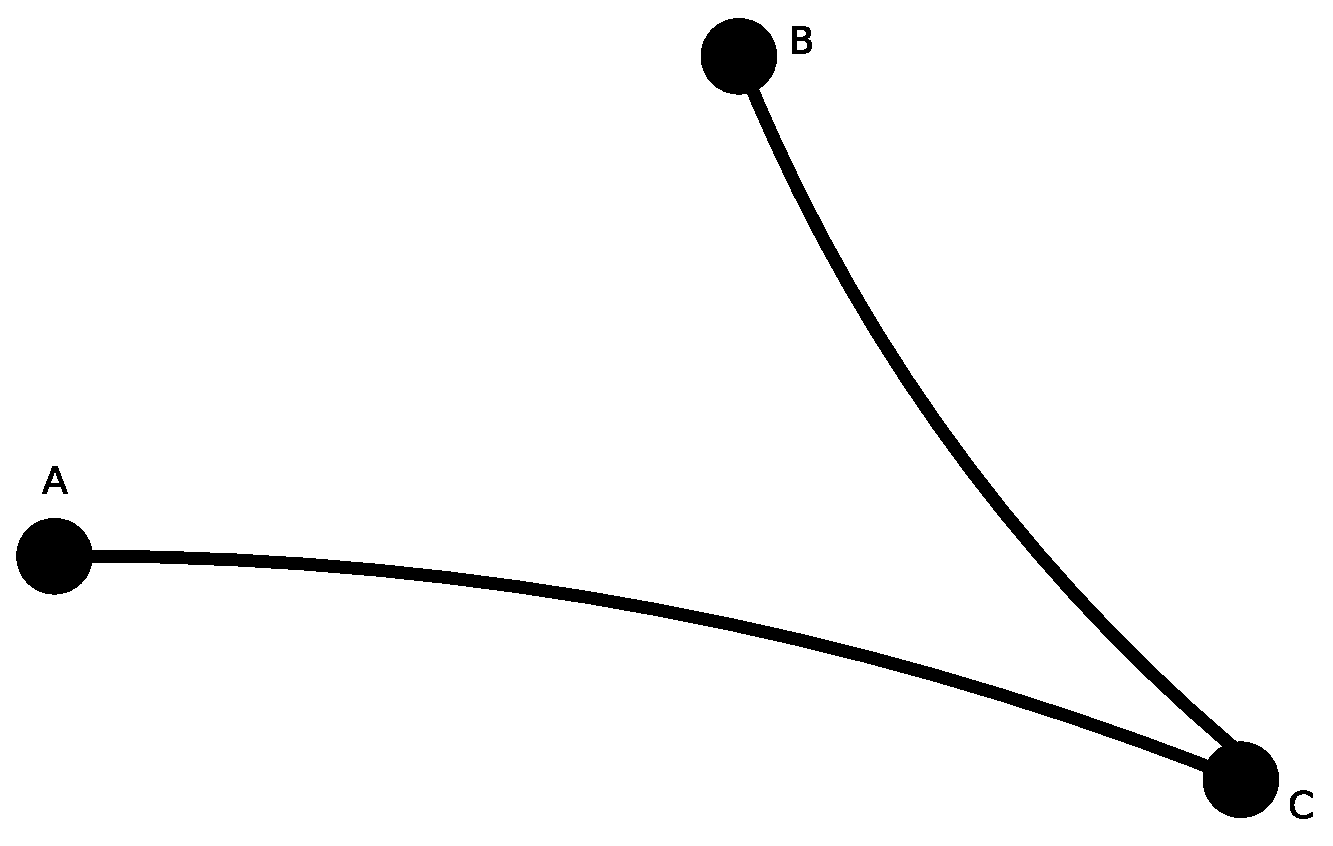
\includegraphics[height=1.5in]{k3_notmax}
\caption{This graph is not maximally planar because one can extend the graph to $K_3$, a larger, planar graph, by adding an edge connecting vertex a and b.}
\label{fig4}
\end{figure}

We leave out the proof for the following classical result.
\begin{lemma}\label{planarn3}
%\begin{enumerate}
%\item{Every maximal plane graph is maximally planar}
%\item{A planar graph with $n\geq 3$ vertices is maximally planar if and only if it has $3n-6$ edges.}
%\end{enumerate}
A planar graph with $n\geq 3$ vertices is maximally planar if and only if it has $3n-6$ edges.
\end{lemma}


%%%%%%%%%%%%%%%%%%%%%%%%%%%%%%%%%%%%%%%%%%%%%%%%%%%%%%%%%%%%%%%%%%%%%%%%%%%%%%%%%%%%%%%%%%%%%%%%%%%%%%%%%%%
\subsection{Euler's formula}
Euler's formula may be used to describe plane graphs. We omit the proof of the Euler's formula, shown below.
\begin{theorem}
Let G be a connected plane graph with $n$ vertices, $m$ edges, and $l$ faces. Then 
$$n-m+l=2.$$
\end{theorem}

\begin{corollary}\label{coro_euler}
A plane graph with $n \geq 3$ vertices has at most 3n-6 edges. Every plane triangulation with n vertices has 3n-6 edges. 
\end{corollary}
\begin{proof}
In a plane triangulation $G$, every face boundary contains exactly three edges, and every edge lies on the boundary of exactly two faces. Let $E(G)$ be the edge set of $G$ and let $F(G)$ be the face set of $G$. The bipartite graph on $E(G) \cup F(G)$ has edge set $\{ef | e \subseteq G[f]\}$ and there it has exactly $2|E(G)| = 3|F(G)|$ edges. We take Euler's formula and replace $l$ with $2m/3$ to get:
$$n - m +2m/3 = 2$$ which evaluates to $$m=3n-6.$$
\end{proof}

We can use Euler's formula to show whether or not a given graph can be shown as a plane graph. For example, the graph $K_5$ has $n=5, m=10, l=6$. $K_5$ is not a plane graph because the number of edges is 
$$10 > 3(5) - 6,$$
therefore contradicting the corollary of the theorem. Likewise $K_{3,3}$ cannot occur as a plane graph and that can be shown with Euler's theorem.

The following will be instrumental in showing the conditions under which a graph is considered planar.

\begin{corollary}\label{corollary-euler}
A plane graph does not contain $K_5$ or $K_{3,3}$  as a topological minor.
\end{corollary}

%The meaning of Corollary \ref{corollary-euler} will become more clear after reading section \ref{kuratowski}, which discusses Kuratowski's Theorem.

%%%%%%%%%%%%%%%%%%%%%%%%%%%%%%%%%%%%%%%%%%%%%%%%%%%%%%%%%%%%%%%%%%%%%%%%%%%%%%%%%%%%%%%%%%%%%%%%%%%
\section{Proof of Corollary \ref{corollary-euler} using Euler's Rule}
\begin{proof}
Since a planar graph is also a plane graph, then Corollary \ref{coro_euler} can be applied to planar graphs. Let $G$ be a planar graph. Assume that $G$ has a $K_5$ as a minor. Since $G$ is planar, then Corollary \ref{coro_euler} must apply to all minors of G. Applying the formula with the number of vertices of $K_5$, $n=5$, and the number of edges, $m=10$, we find that the number edges, would need to satisfy
$$10 > 3(5) - 6,$$ which evaluates to false. This contradicts the statement that $G$ is planar, and therefore we conclude that a graph with a $K_5$ minor is non-planar.

Next, assume that $G$ has a $K_{3,3}$ minor. We apply Corollary \ref{coro_euler}, with the number of vertices in $K_{3,3}$, $n=6$ and the number of edges $m=9$. Therefore the following would need to evaulate true:
$$9 > 3(5) - 6.$$
Since the statement evaluates false, this contradicts the claim that the graph is planar. Thus, we conclude that a graph with a $K_{3,3}$ minor is non-planar.
\end{proof}





%%%%NEW Kuratowski
\section{Kuratowski's Theorem}
In this section we will prove Kuratowski's theorem, which implies that a graph is planar if it does not contain $K_5$ or $K_{3,3}$ as a topological minor. A graph H is called a \emph{topological minor} of a graph $G$ if a subdivision of $H$ is isomorphic to a subgraph of $G$. Let $TK_5$ be the $K_5$ topological minor. That is, the $K_5$ graph can be obtained by contracting certain edges in a subgraph of $G$. Similarly, let $TK_{3,3}$ be the $K_{3,3}$ topological minor. A graph $H$ is called a \emph{minor} of the graph $G$ if $H$ is isomorphic to a graph that can be obtained by zero or more edge contractions on a subgraph of $G$. Let $MK_5$ be the minor of a graph $G$ that is $K_5$. Let $MK_{3,3}$ be the minor of a graph $G$ that is $K_{3,3}$. 

Formally, Kuratowski's Theorem is as follows.
\begin{theorem}
The following assertions are equivalent for graph G:
\begin{enumerate}[(i)] 
\item{$G$ is planar;}
\item{$G$ contains neither $TK_5$ nor $TK_{3,3}$;}
\item{$G$ contains neither $MK_5$ nor $MK_{3,3}$.}
\end{enumerate}
\end{theorem}

We first show that topological minors of $K_5$ and $K_{3,3}$ contain minors of $K_5$ and $K_{3,3}$. Next we show that any 3-connected graph is planar if it does not contain $K_5$ or $K_{3,3}$ as a minor. Afterwards we use induction to show that a graph $G$ with $|G| > 4$ that is edge-maximal and does not have a $TK_5$ or $TK_{3,3}$, is 3-connected. This allows us to generalize any large graph without $K_5$ or $K_{3,3}$ minors as 3-connected, and therby non-planar.

\begin{lemma}\label{lemma4.2.6}
In a 2-connected plane graph, every face is bounded by a cycle.
\end{lemma}

\begin{lemma}\label{lemma3.2.4}
Every 3-connected graph $G\neq K_4$ has an edge $e$ such that $G/e$ is again 3-connected.
\end{lemma}
\begin{proof}
Suppose such an edge $e$ does not exist. Then, for each edge in $G$, there is a separator $S$ of at most 2 verices. Suppose the contracted vertex $v_{xy}$ of $G/xy$ lies in $S$ and $|S| = 2$. If this is the case, then there should be another vertex $z$ , $z \notin \{x,y\}$ such that $\{v_{xy},z\}$ separates $G/xy$. Then, any two vertices separatec by $\{v_{xy},z\}$ would also be separted in $G$ by $T:=\{x,y,z\}$. Every vertex in the set $T$ has a neighbor in every component $C$ of $G - T$. 

For a component $C$, choose the edge $xy$, the vertex $z$, and a neighbor $v$ of $z$ in $C$, so that $|C|$ is as small as possible. The graph $G/zv$ will not be 3-connected, and therefore there exists a vertex $w$ such that $\{z,v,w\}$ separates $G$, and therefore every vertex in $\{z,v,w\}$ has a neighbor in every component of $G - \{z,v,w\}$. 

The graph $G - \{z,v,w\}$ has a component $D$ such that $D \cap \{x,y\} = \varnothing$. If this is the case then every neighbor of $v$ in $D$ also is contained in $C$, because $v$ is in $C$. It follows that $D \cap C \neq \varnothing$, and $D \subsetneq C$ by the choice of $D$. This contradicts the choice of $xy, z$ and $C$.
\end{proof}

\begin{proposition}\label{prop1.7.4}
\begin{enumerate}[(i)]
\item{Every topogical minor of a graph contains a minor.}
\item{If the degree of a graph X, $\Delta(X) \leq 3$, then every minor of X is also the graph's topogical minor.}
\end{enumerate}
\end{proposition}

\begin{lemma}\label{minor_topoMinor}
A graph $G$ contains $K_5$ or $K_{3,3}$ as a minor if and only if it contains $K_5$ or $K_{3,3}$ as a topological minor. That is, $G$ has $MK_5$ or $MK_{3,3}$ if and only if $G$ has $TK_5$ or $TK_{3,3}$. 
\end{lemma}
\begin{proof}
Let $G$ be a graph that has a $TK_5$ or $TK_{3,3}$. In this case, $G$ has a $MK_5$ or $MK_{3,3}$ by Proposition \ref{prop1.7.4}. 

Conversely, let $G$ have a $MK_5$ or $MK_{3,3}$. Two cases can follow:

\emph{Case 1: $G$ has a $MK_{3,3}$}. Since $\Delta(X) \leq 3$, we have (by Proposition \ref{prop1.7.4}) that $G$ has a $TK_{3,3}$. See Figure \ref{minor_topoMinorCase1}.

\begin{figure}[htbp]
	\centering
	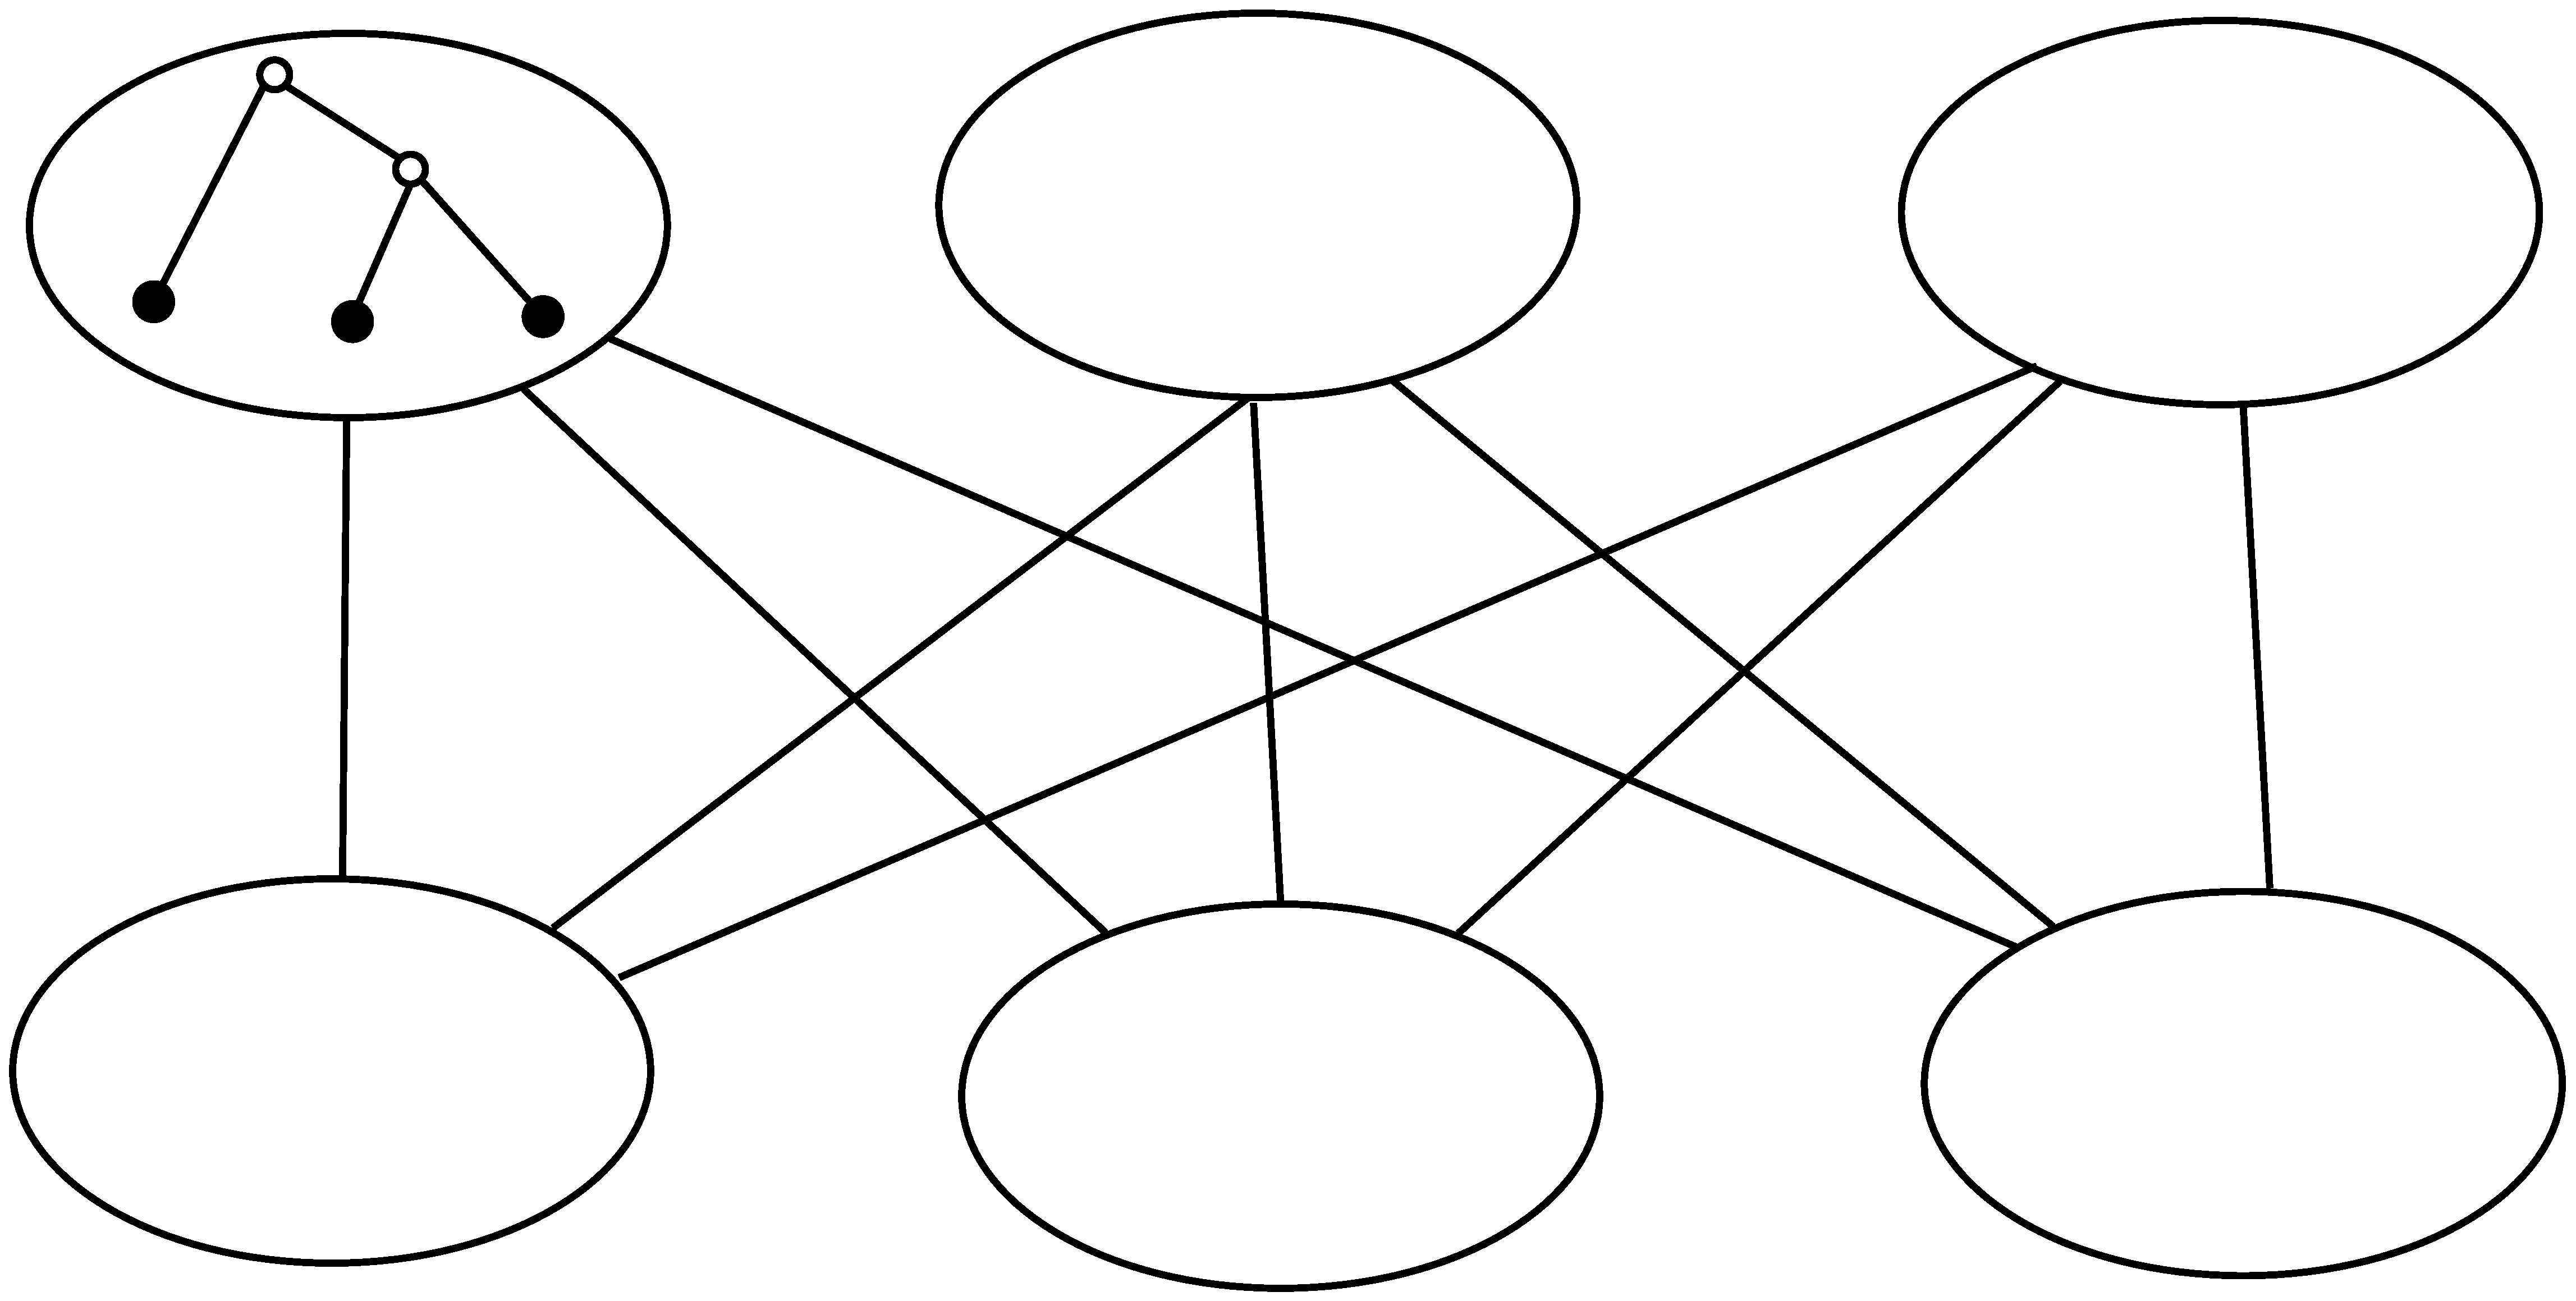
\includegraphics[height=2in]{minor_topoMinorCase1.eps} \\ 
	\caption{Lemma \ref{minor_topoMinor}, Case 1: This graph has $MK_{3,3}$, since  $\Delta(X) = 3$ and since the tree in the upper left corner can be contracted to a single vertex of the graph $K_{3,3}$. If we start with a $K_{3,3}$ graph, a subdivision of the edges connected to the vertex in the top left yields the graph G. Therefore, there is a $TK_{3,3}$ in the graph G.}
\label{minor_topoMinorCase1}
\end{figure}

\emph{Case 2: $G$ has a $MK_5$}. In this case we will be able to find either $TK_5$ or $TK_{3,3}$ in the graph. If each branching set of the $MK_5$ has $TK_{1,4}$ or $TK_{1,3}$ or $TK_{1,2}$, with endpoints $s_i$, then $G$ has a $TK_5$. See example in figure \ref{minor_topoMinorCase2}A.

\begin{figure}[htbp]
	\centering
	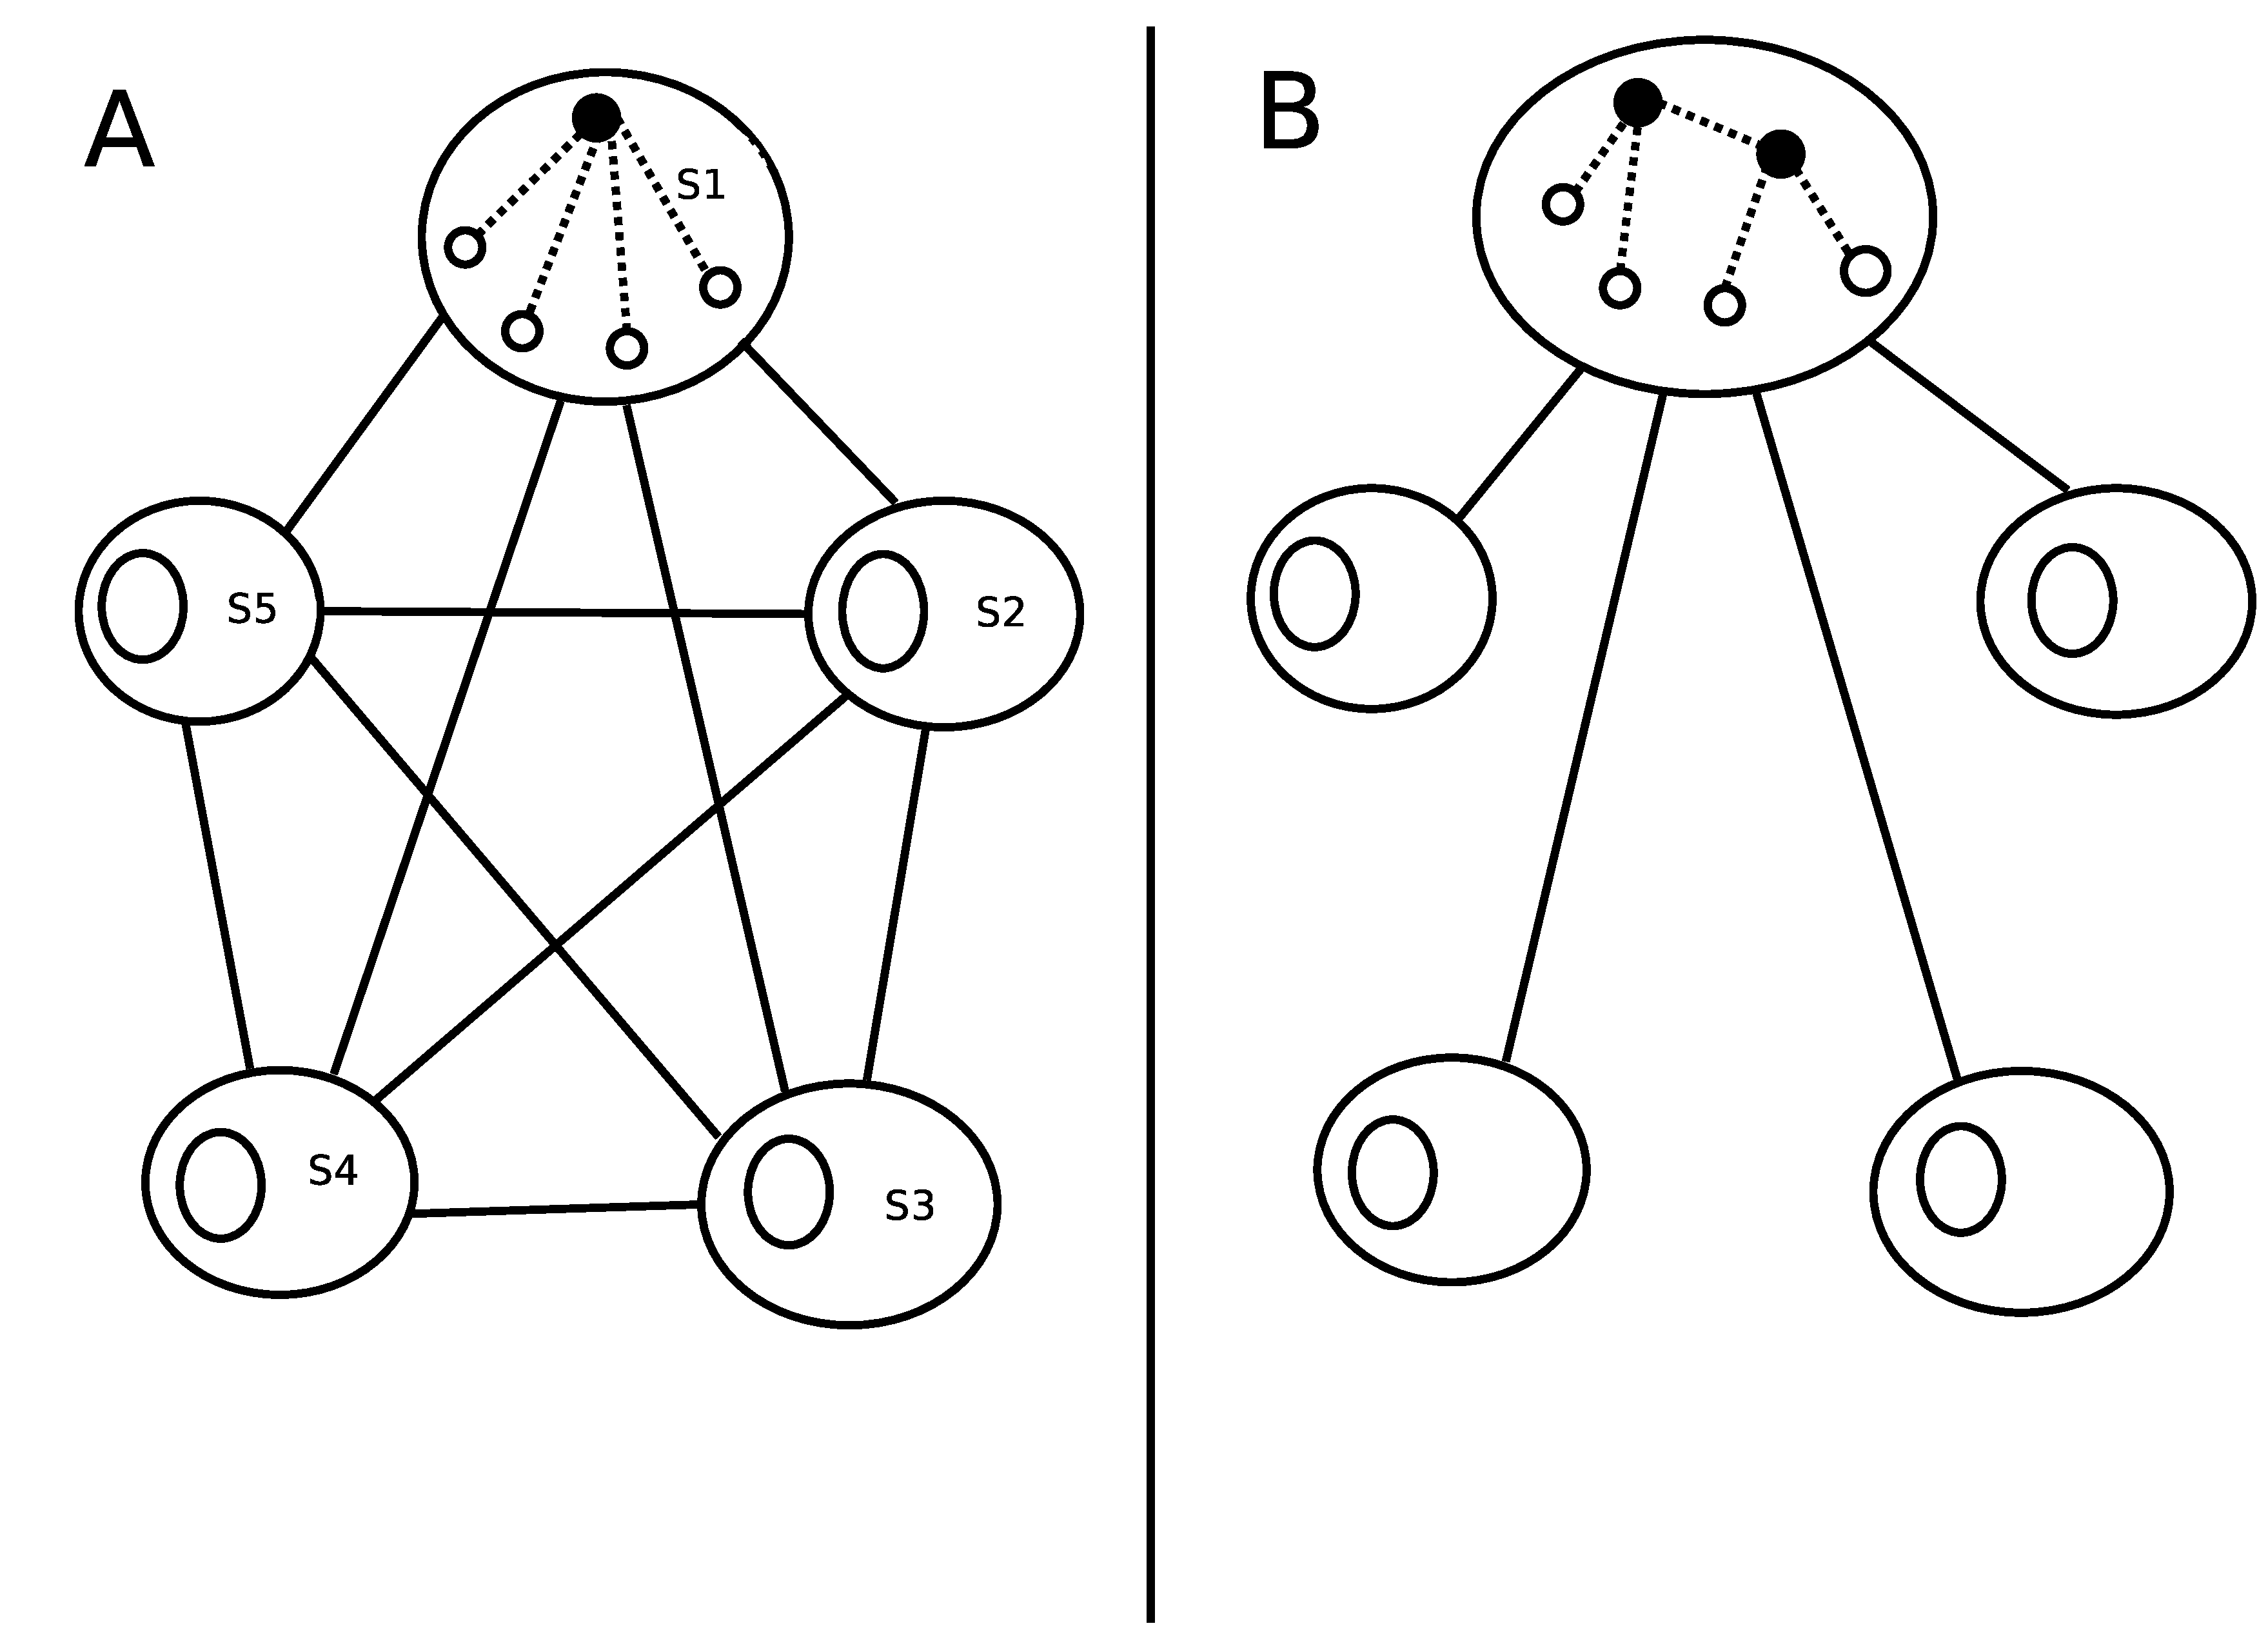
\includegraphics[height=4.5in]{minor_topoMinorCase2.eps} \\ 
	\caption{Lemma \ref{minor_topoMinor}, Case 2. A)$s_i$ for $i=1,..5$ are the vertices of the $TK_5$. B) $TK_{3,3}$ is formed by vertices $x,y,u_1,u_2,u_3,u_4$.}
\label{minor_topoMinorCase2}
\end{figure}

On the other hand, if there exists a branch set in $G$ such that $TK_{1,4}$ does not exist, then the graph has two vertices of degree 3. Let the vertices of each of the five branch sets be contracted to these two vertices of degree 3. Furthermore, contract every other branch set to a single vertex. We would them obtain a graph on 6 vertices that contains $K_{3,3}$. See example in figure \ref{minor_topoMinorCase2}B.
\end{proof}





The heart of the proof lies in Lemma \ref{planar}, below.
\begin{lemma}\label{planar}
Every 3-connected graph G without a $K_5$ or $K_{3,3}$ minor is planar. 
\end{lemma}

\begin{proof}
We consider a 3-connected graph $G$ without a $MK_5$ or a $MK_{3,3}$. We want to prove that $G$ is planar. For set of vertices of a graph G, we apply induction on $|V(G)|$. The base case for the induction is $|v(G)|=4$. The only such 3-connected graph where $|v(G)|=4$ is the graph $K_4$. The assertion still holds for $K_4$, which is planar. See figure \ref{k4_plane}. It is easy to see (by brute force) that the assertion holds true for smaller graphs where $|v(G)|<4$.  Next, we consider all cases where $|v(G)| > 4$. 

Suppose now that $|V(G)| > 4$. By Lemma \ref{lemma3.2.4}, there exists an edge $e \in E(G)$ such that $G/e$ is 3-connected. Note that $G/e$ does not contain $MK_5$ or $MK_{3,3}$. (If $G/e$ contained $MK_5$ or $MK_{3,3}$, then $G$ would have contained those). Let $G':=G/e$. Let $e = xy$, the edge connecting vertices $x$ and $y$. Let $v_{xy}$ represent the vertex that results from the contraction of edge $e = xy$ in graph $G'$. The graph $G'$ is planar. Thus, $G'$ can be drawn in the plane without edge crossings.

Let $f$ be the face in $G' - v_{xy}$ containing $v_{xy}$, and let $C$ be the boundary of $f$. Let $X:=N_G(x)$ be the set of neighbors of $x$ in $C$. Similarly, let $Y:=N_G(y)$ be the set of neighbors of $y$ in $C$. The verties of $C$ are such that $X \cup Y \subseteq V(C)$. We can derive the graph 
$$G'*:= G' - \{v_{xy}v | v \in Y \backslash X\},$$
which is the graph $G'$ with the following edges removed: edges that connect $y$ with vertices in $C$ that are not in $X$, removed. See figure \ref{GprimeStar}.
\begin{figure}[htbp]
	\centering
	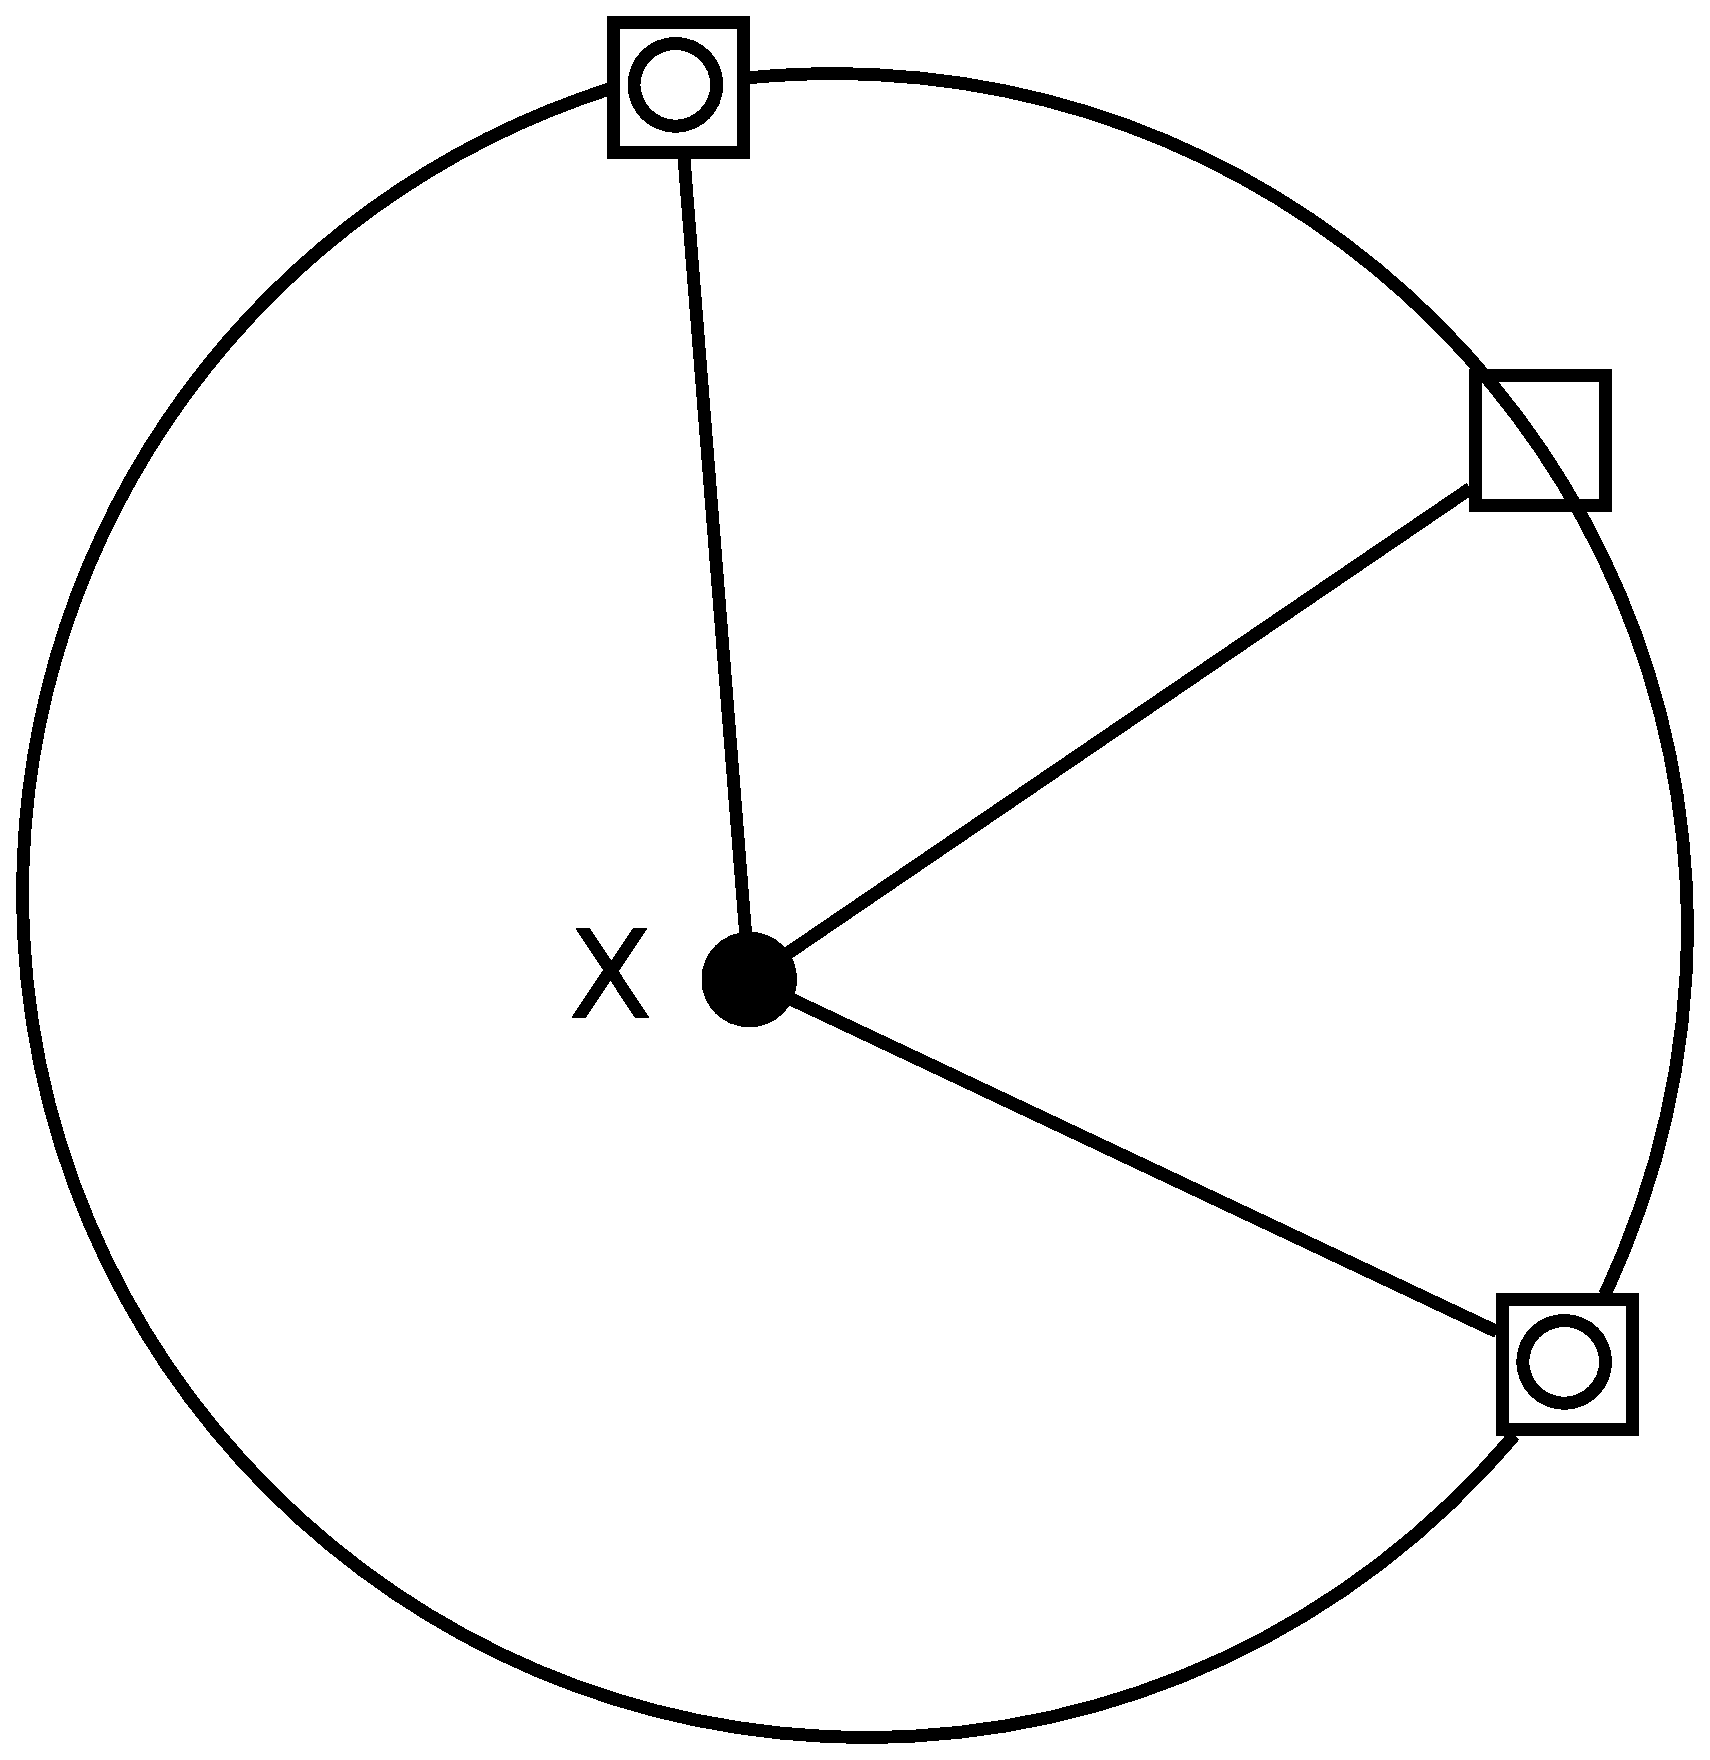
\includegraphics[height=2in]{GprimeStar} \\ 
	\caption{The graph $G'*$ which is obtained by removing from $G'$ the edges that connect $y$ with vertices in $C$ that are not connected to $x$. The cycle $C$ is comprised of the vertices that are the neighbors of $x$ and $y$. The boundary for $C$ is shown on this graph; however, note that the boundary shown in $G'*$ does not contain the vertices of $Y$.}
\label{GprimeStar}
\end{figure}

The graph $G'*$ may be viewed the same way as $G - y$, in which the vertex $x = v_{xy}$. In $G - y$, we seek to add back the vertex $y$ and the deleted edges in order to obtain a drawing of G. Another way to think about this is to think about uncontracting $v_{xy}$ in the graph $G'$ in order to form $G$.  Since $G'$ is 3-connected, and $G'-v_{xy}$ is 2-connected, then $C$ is a cycle by Lemma \ref{lemma4.2.6}.

Next, we will identify all possible cases where we can uncontract $v_{xy}$. Let the vertices in $X$ be numbered $x_1, x_2, ... x_k$ and let $P_i = x_i ... x_{i+1}$ be the set of X-paths on $C$, for $i = 1,...,k$ and $x_{k+1}:=x_1$. For example, the particular path $P_3$ is the path $x_3 ... x_k, x_1$. 

We will show that $Y\subseteq V(P_i)$. First, assume that $Y\not\subseteq V(P_i)$. There are three cases in which this happens.

\emph{Case 1}. %%when none of the X's are contained in Y
For some $i$, $y$ has a neighbor $y' \in P_i$ for some $i$, and $y$ has another neighbor $y'' \in C - P_i$. The vertices $y'$ and $y''$ would be separated in C by $x':=x_i$ and $x'':=x_{i+1}$, such that the vertices are arranged in the order $y'$, $x'$, $y''$,$x''$. In this graph, there exists a $MK_{3,3}$. This contradicts the notion that the graph G is planar. See figure \ref{case1}.

\begin{figure}[htbp]
	\centering
	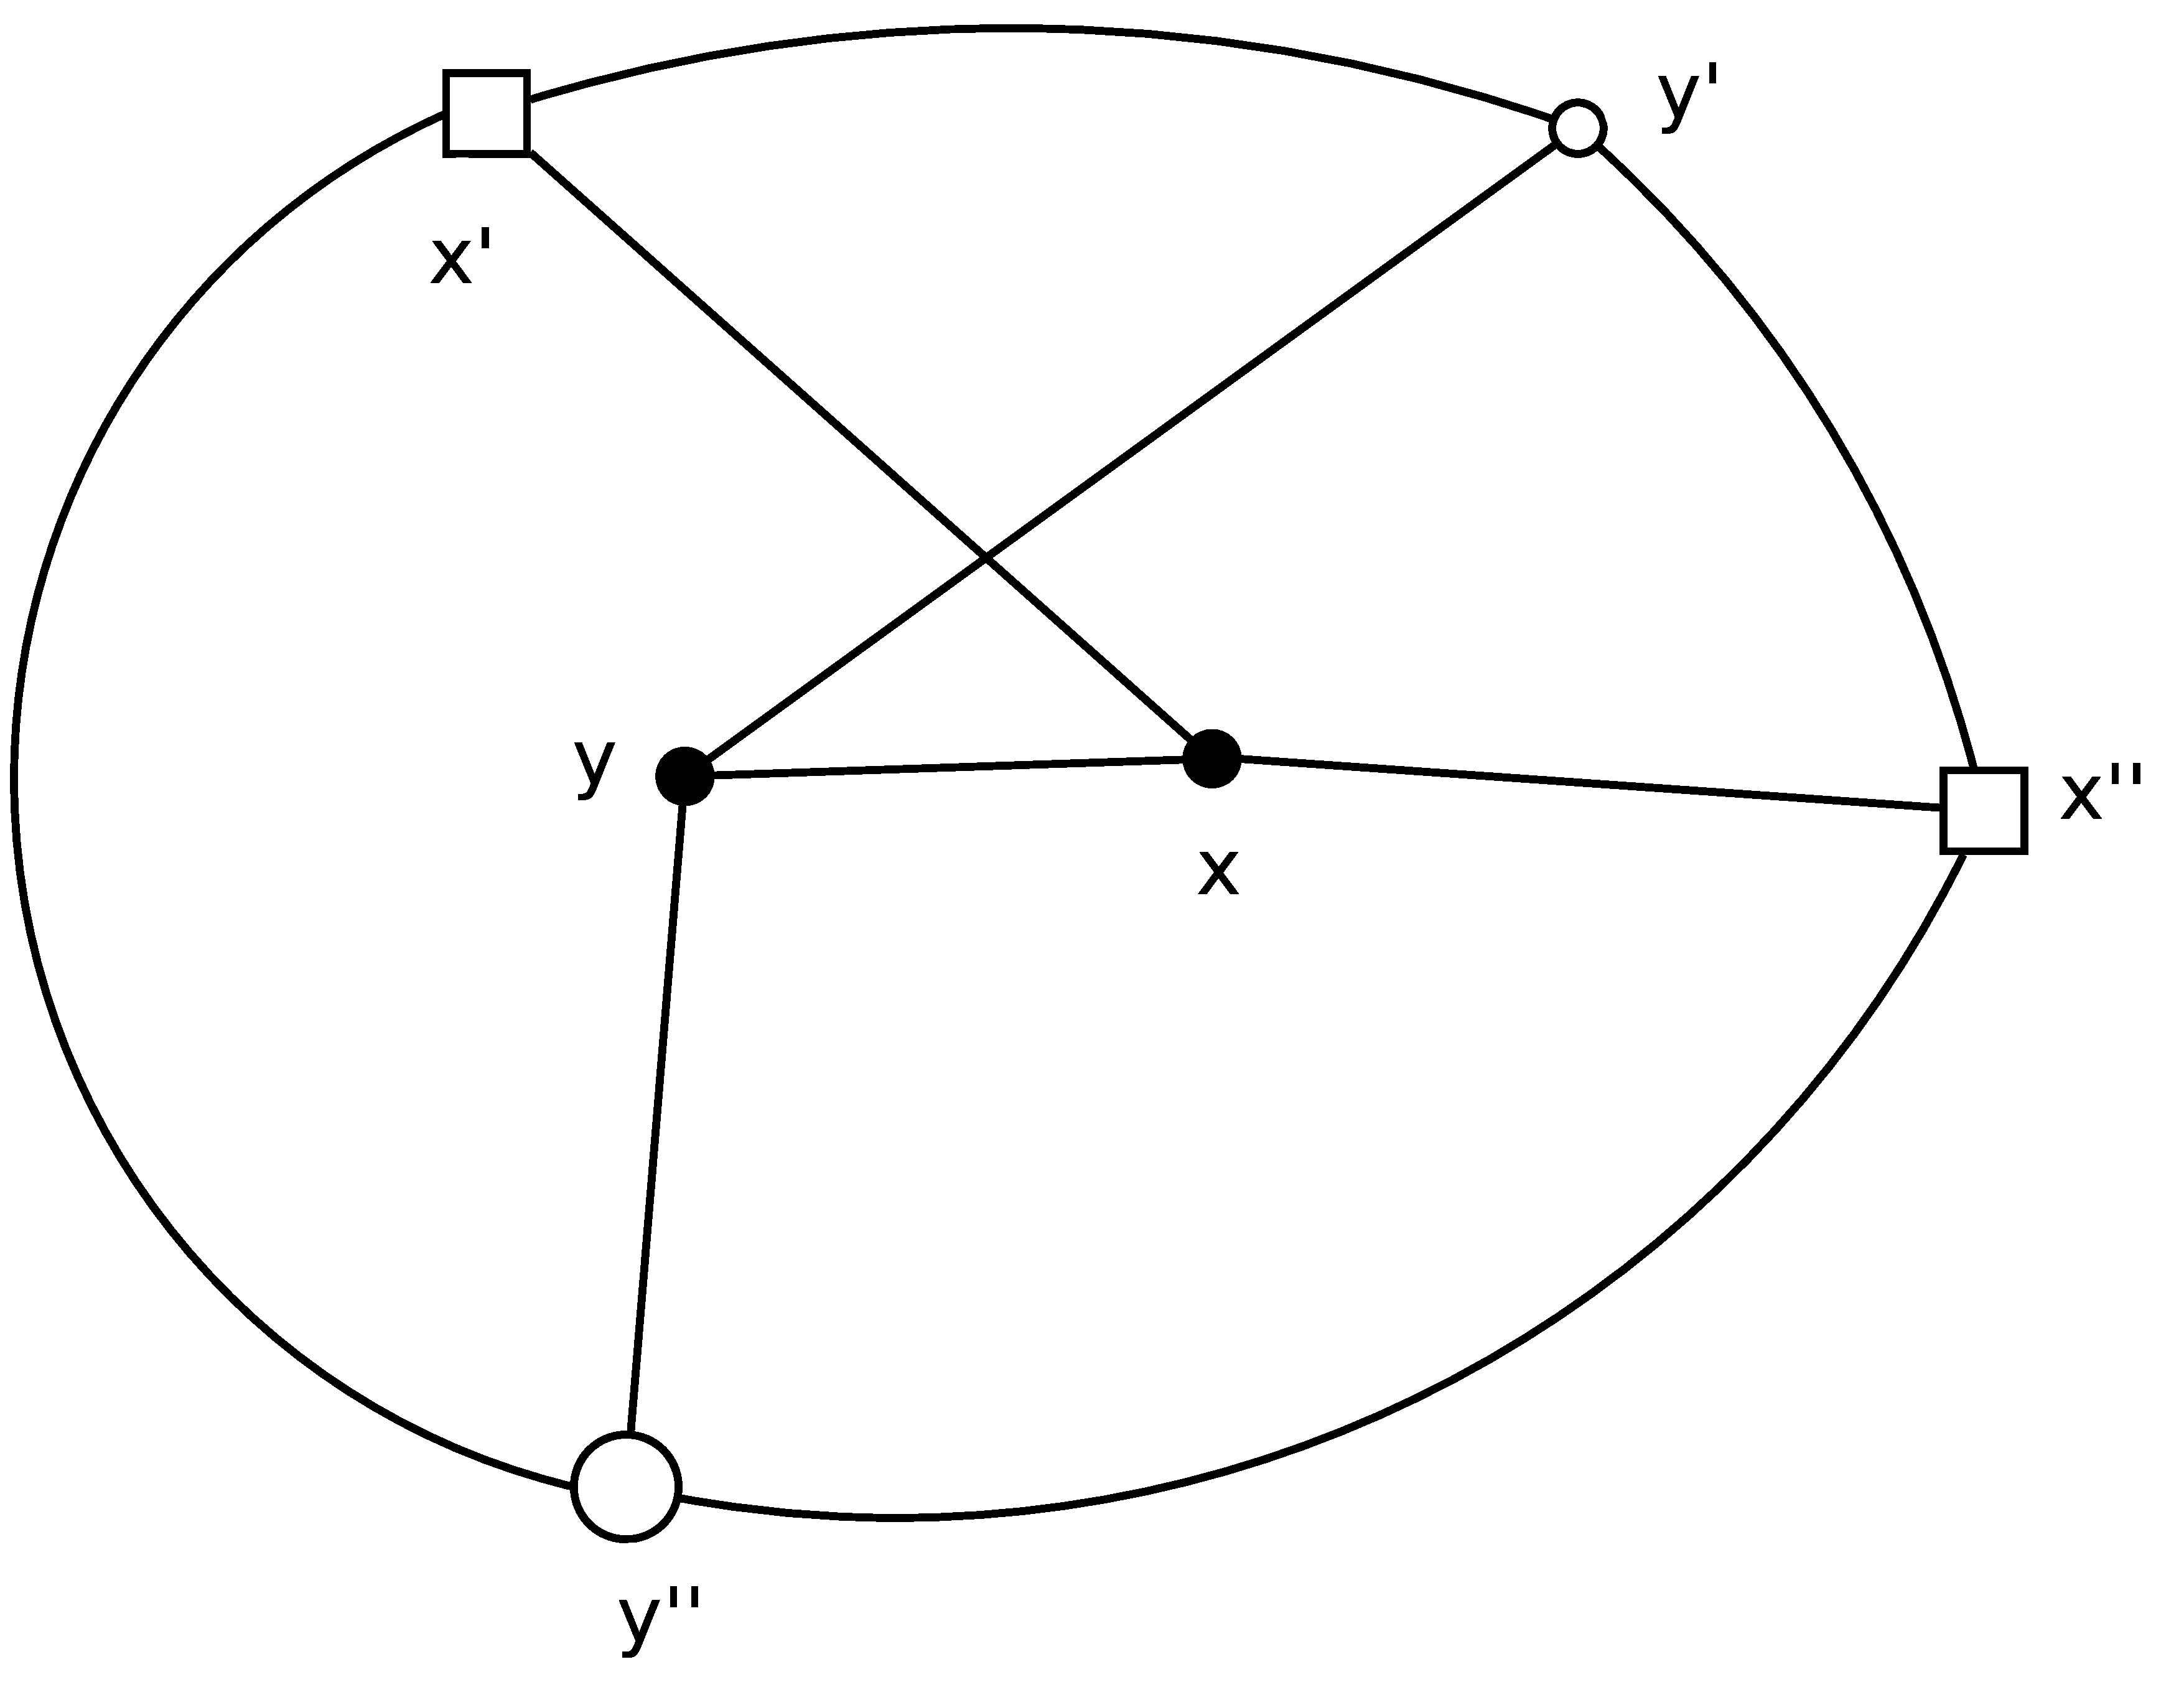
\includegraphics[height=2in]{case1.eps} \\ 
	\caption{Case 1: None of the vertices in Y are contained in X and vice versa. The vertices $y'$ and $y''$ are separated by $x'$ and $x''$, resulting in a $MK_{3,3}$.}
\label{case1}
\end{figure}

\emph{Case 2}. Suppose that $Y \subseteq X$ and $|Y \cap X| \leq 2$. In this case, $y$ has two neighbors, $y'$ and $y''$, on $C$ that do not lie on the same $P_i$. Since they do not lie on the same $P_i$, $y'$ and $y''$ are separated on $C$ by vertices $x', x'' \in X$ and these vertices are arranged in the order $y', x',y'',x''$ on the cycle. As with case 1, in this graph there exists a $MK_{3,3}$. This contradicts the notion that the graph G is planar. See figure \ref{case2}.

\begin{figure}[htbp]
	\centering
	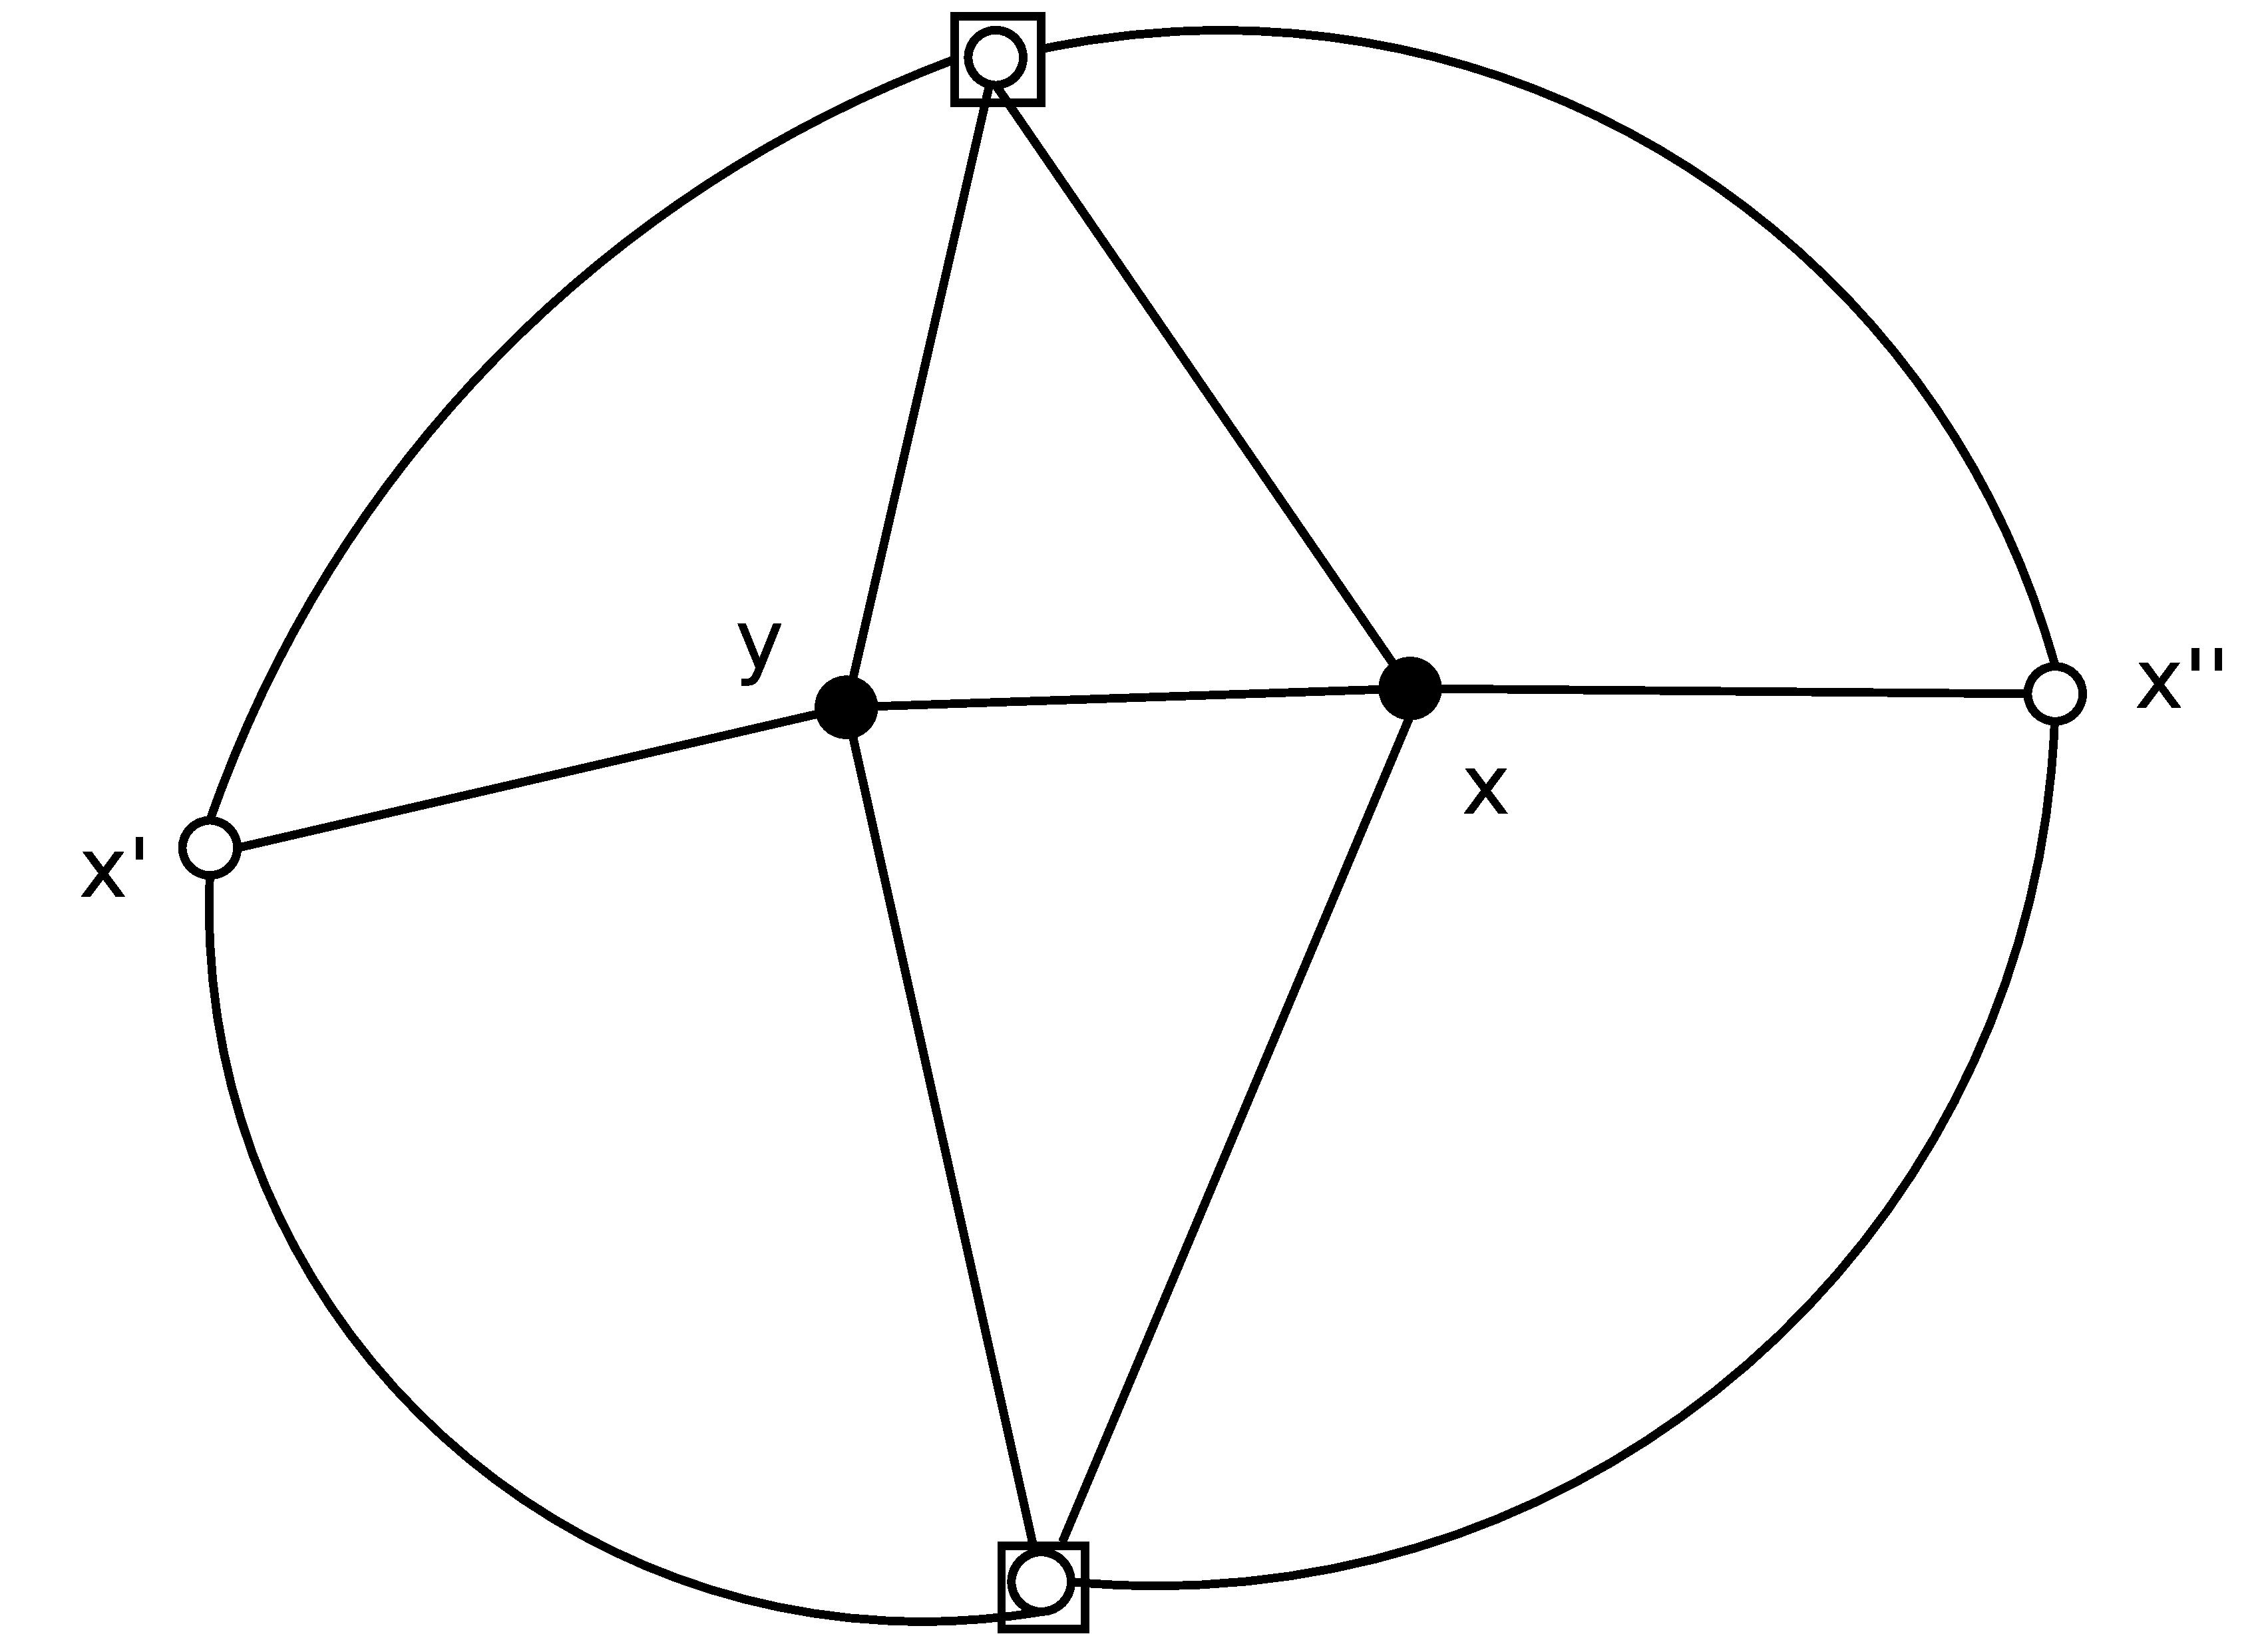
\includegraphics[height=2in]{case2.eps} \\ 
	\caption{Case 2: If $|X\cap Y| = 2$ , and if there are vertices $x'$ and $x''$, then the graph is not planar because it cannot be embedded in the plane without edge crossings. The vertices two sets $x,y',y''$ and $y,x',x''$ form a $MK_{3,3}$.}
\label{case2}
\end{figure}

\emph{Case 3}. Suppose $Y \in X$ and $|Y \cap X| = 3$, in which $x$ and $y$ have three common neighbors on C. In this case, the common neighbors along with $x$ and $y$ form a $MK_5$. This contradicts the notion that the graph G is planar. See figure \ref{case3}.

\begin{figure}[htbp]
	\centering
	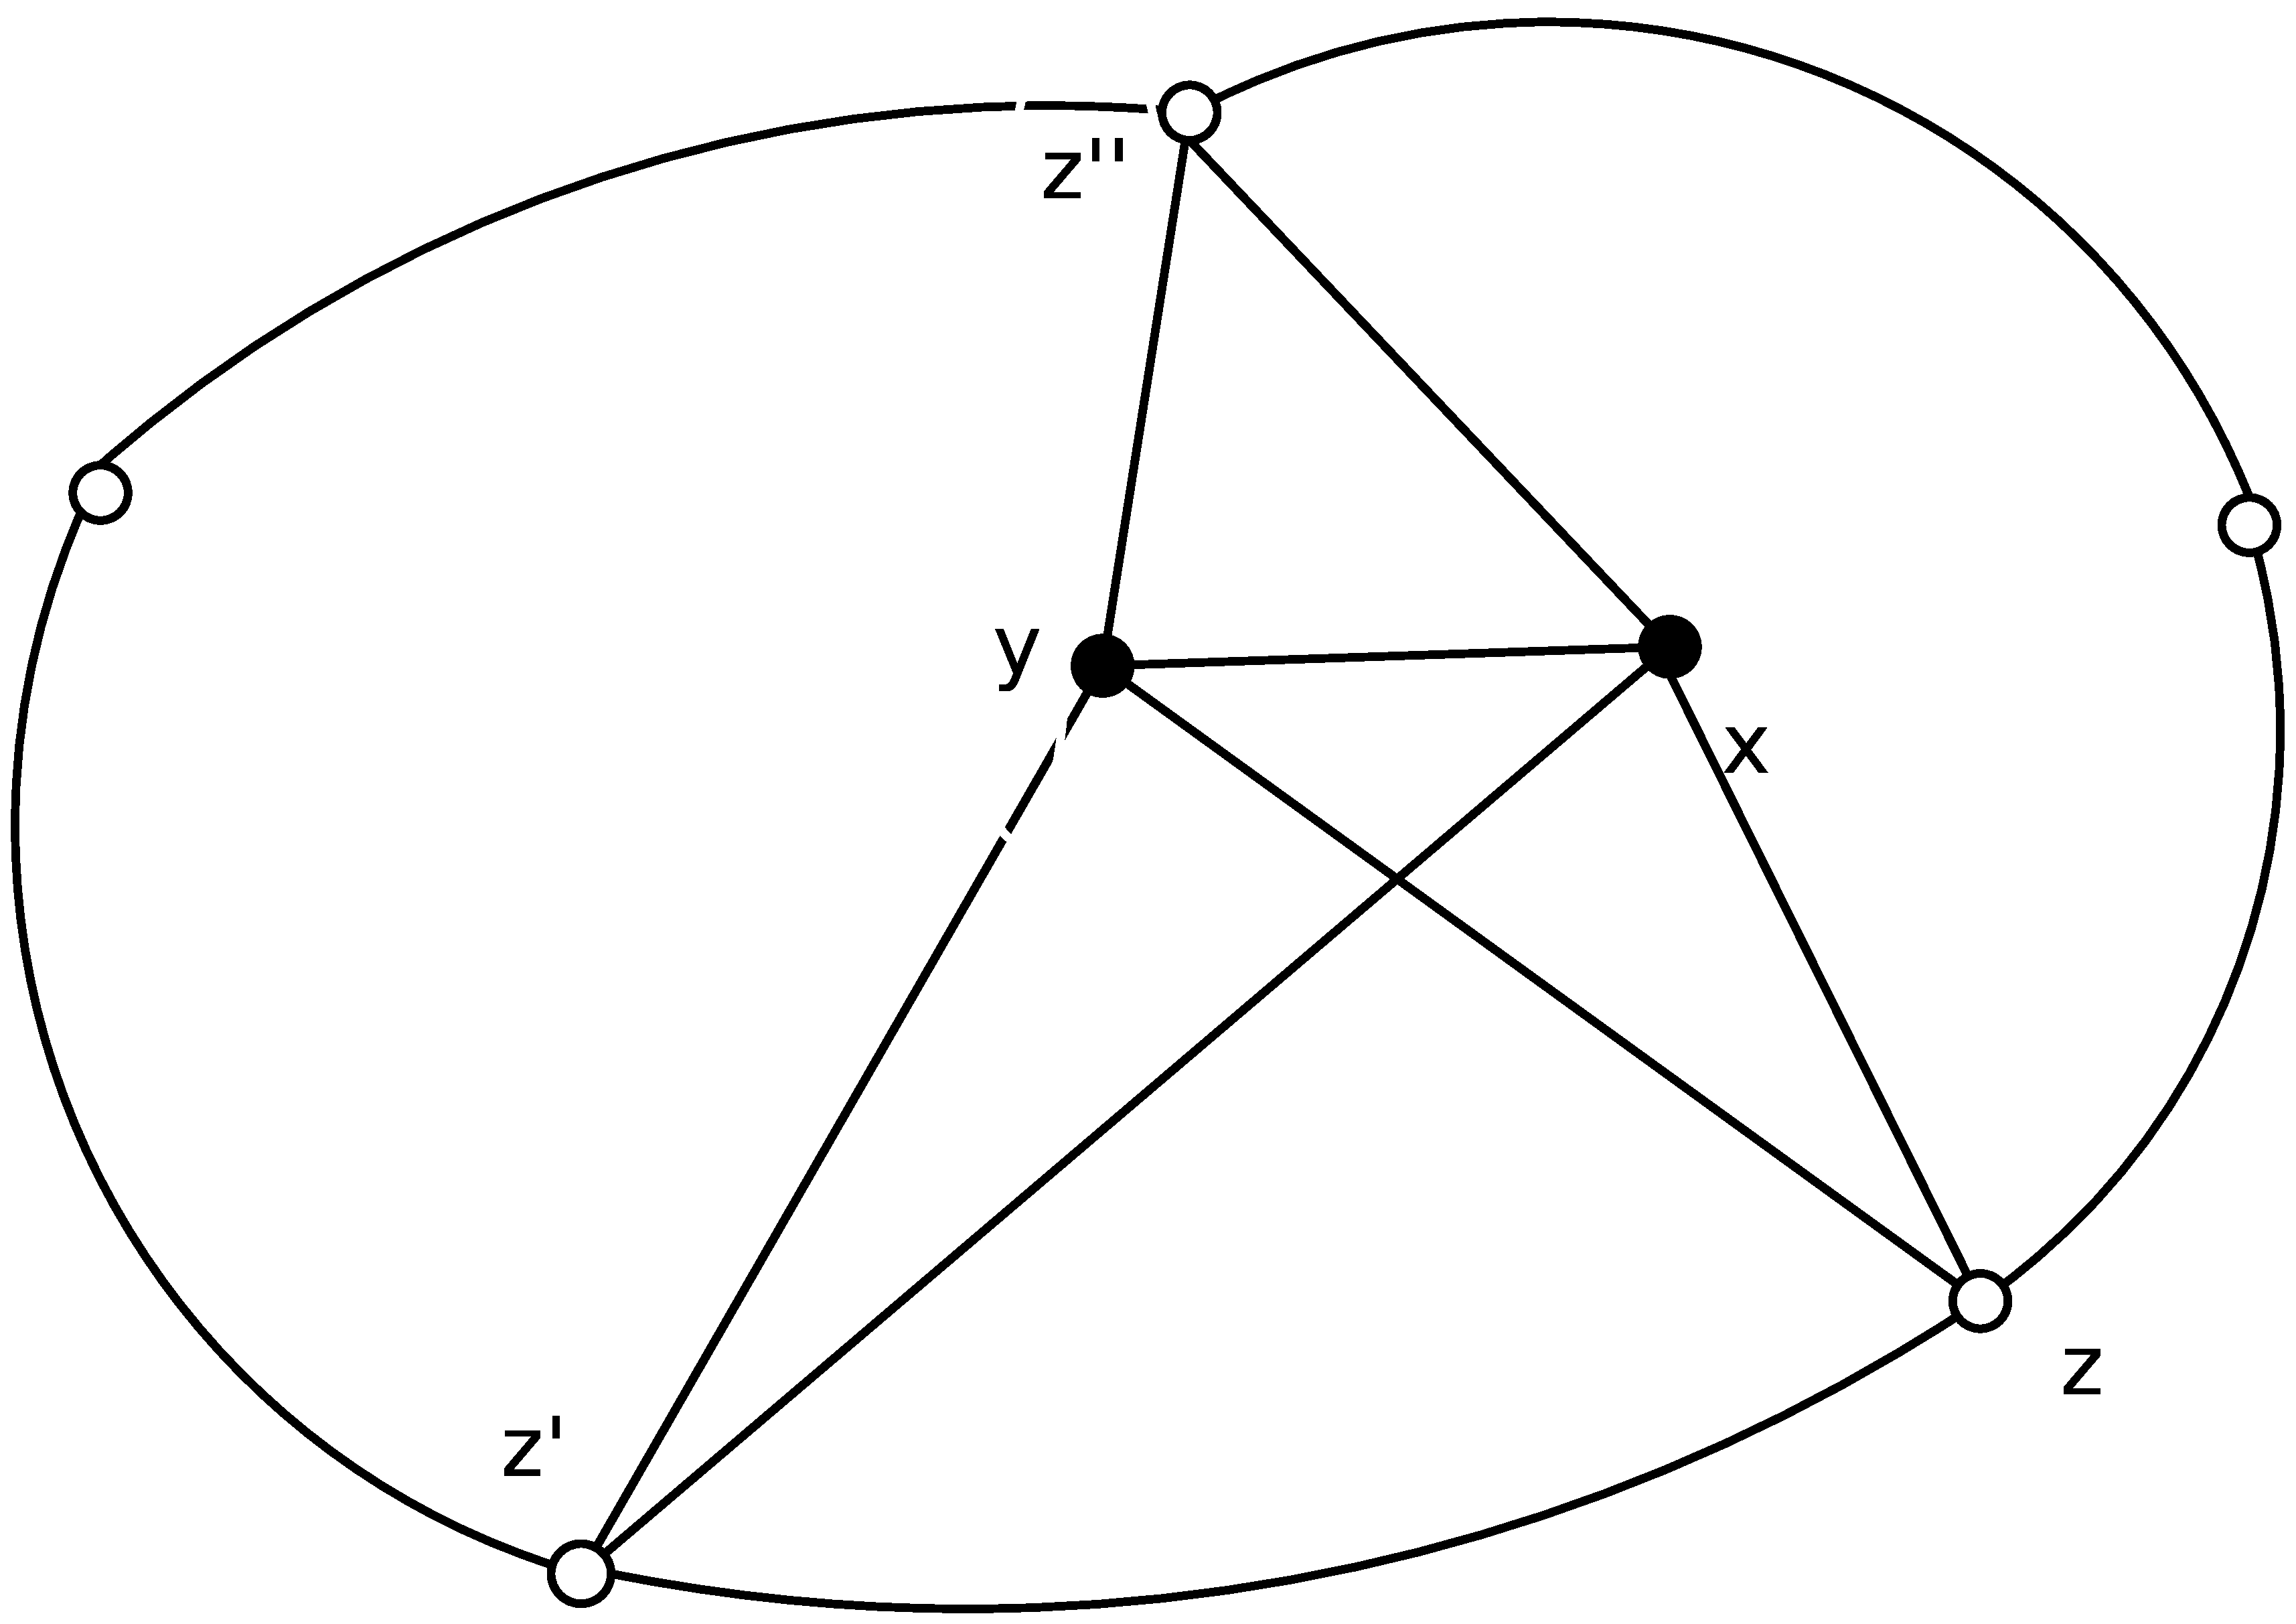
\includegraphics[height=1.5in]{case3.eps} \\ 
	\caption{Case 3: If $x$ and $y$ have three common neighbors $z, z',z''$, then $x,y,z,z',z''$ form a $MK_5$.}
\label{case3}
\end{figure}


We have so far established that, in order for the graph G to be planar, then $Y \subseteq P_i$, for a given $i$. Fix $i$ so that $Y \subseteq P_i$. The set $C \backslash P_i$ is contained in one of the two faces of cycle $C_i:= x x_i P_i x_{i+1} x$, a path which starts at $x$, gets connected to $x_i$, goes through path $P_i$, and connects back to $x$ afterwards. Let the face $f_i$ be the face that is bounded by $C_i$. The face $f_i$ contains points of $f$ but does not contain points of $C$. Thus, $f_i \subseteq f$. (If we refer back to the graph $G'*$, we can see that $f_i$ would only contain the point $x$). 

So what about the edges $xx_j$ that connect $x$ to the vertices in $X$ that are not part of the path $P_i$? These edges meet the cycle $C_i$ only at $x$, and they extend to points $x_j$ that are located in $C\backslash P_i$ (on cycle $C$ but not on cycle $C_i$). Furthermore, the vertices $x_j$ are located outside of $f_i$. This implies that $f_i$ does not contain any edges going through it.

It follows that $f_i \subseteq \mathbb{R}^2 \backslash G'*$. This implies that $f_i$ is contained in a face of $G'*$. Since $f_i$ is contained in a face of $G'*$ (remember, there are no edges running through a face), we can add $y$ to $f_i$, and add the associated edges inside $f_i$ as well. The added edges will not cross any edges associated with $X \backslash Y$, which are not contained in $f_i$ (see figure \ref{faceAdd}).
\end{proof}
\begin{figure}[htbp]
	\centering
	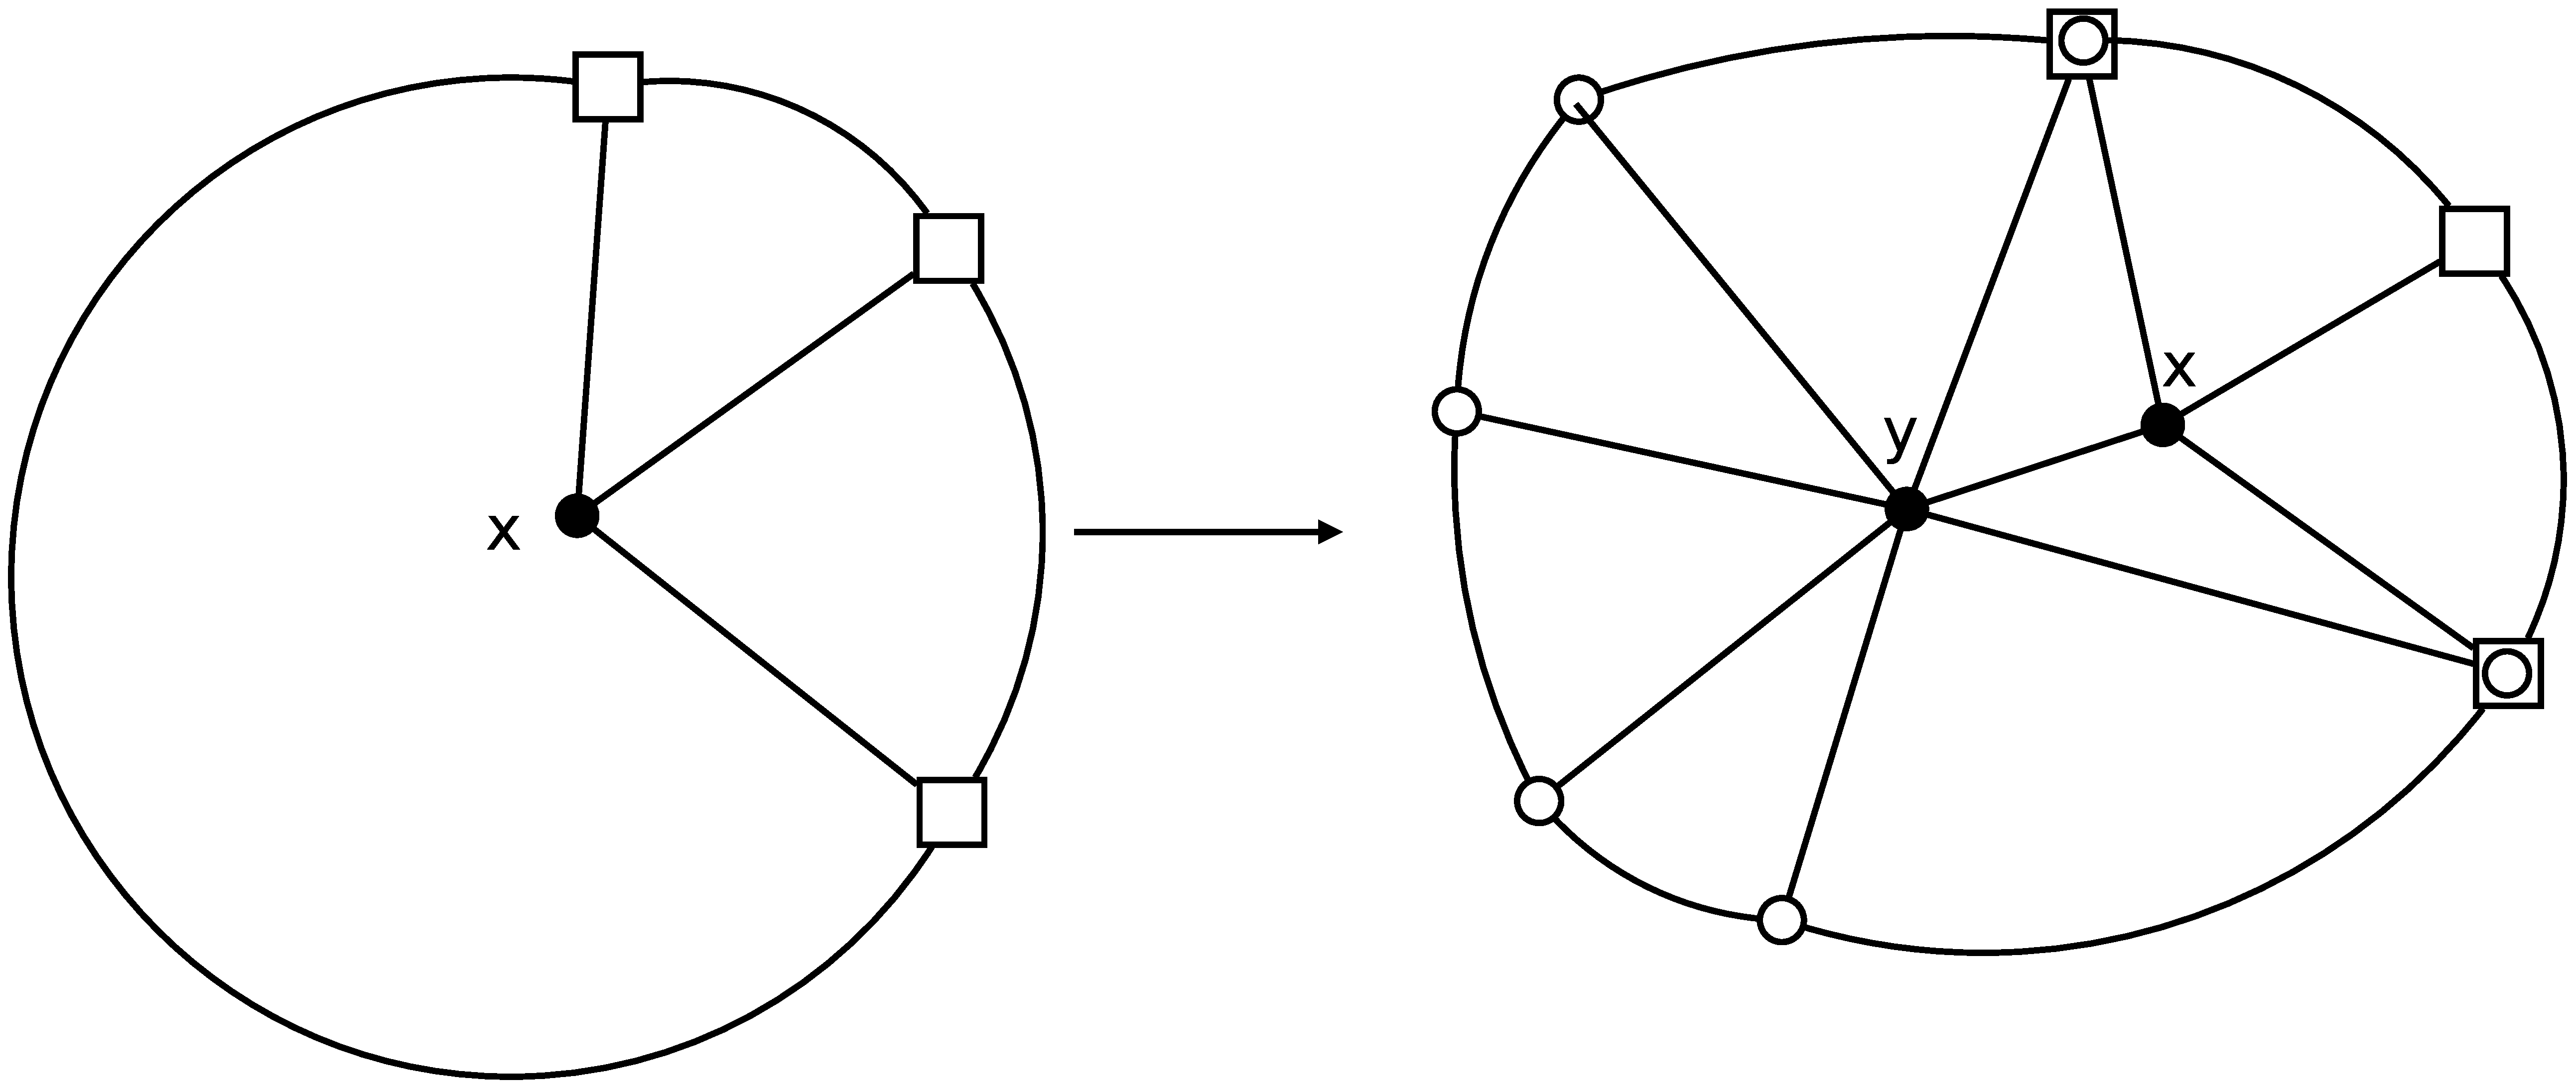
\includegraphics[height=2in]{faceAdd.eps} \\ 
	\caption{The vertex $y$ will be added to the $G'*$ in the face $f_i$ of the graph $G'*$. In the graph $G$, the shaded area corresponds to the face $f_i$ in $G'*$. When the vertex $y$ and its edges can be added to the face $f_i$ of $G'*$, then the graph $G$ is planar.}
\label{faceAdd}
\end{figure}


\begin{lemma}\label{lemma4.4.4}
	\centering
Let $\chi$ be a set of 3-connected graphs. Let G be a graph with a proper separation {$V_1$, $V_2$} of order $\kappa(G)\leq 2$. If $G$ is edge-maximal without a topological minor in $\chi$, then so are $G_1:=G[V_1]$ and $G_2:=G[V_2]$, and $G_1 \cap G_2 = K_2$. (See figure \ref{figLemma4.4.4}).
\end{lemma}
\begin{figure}[htbp]
	\centering
	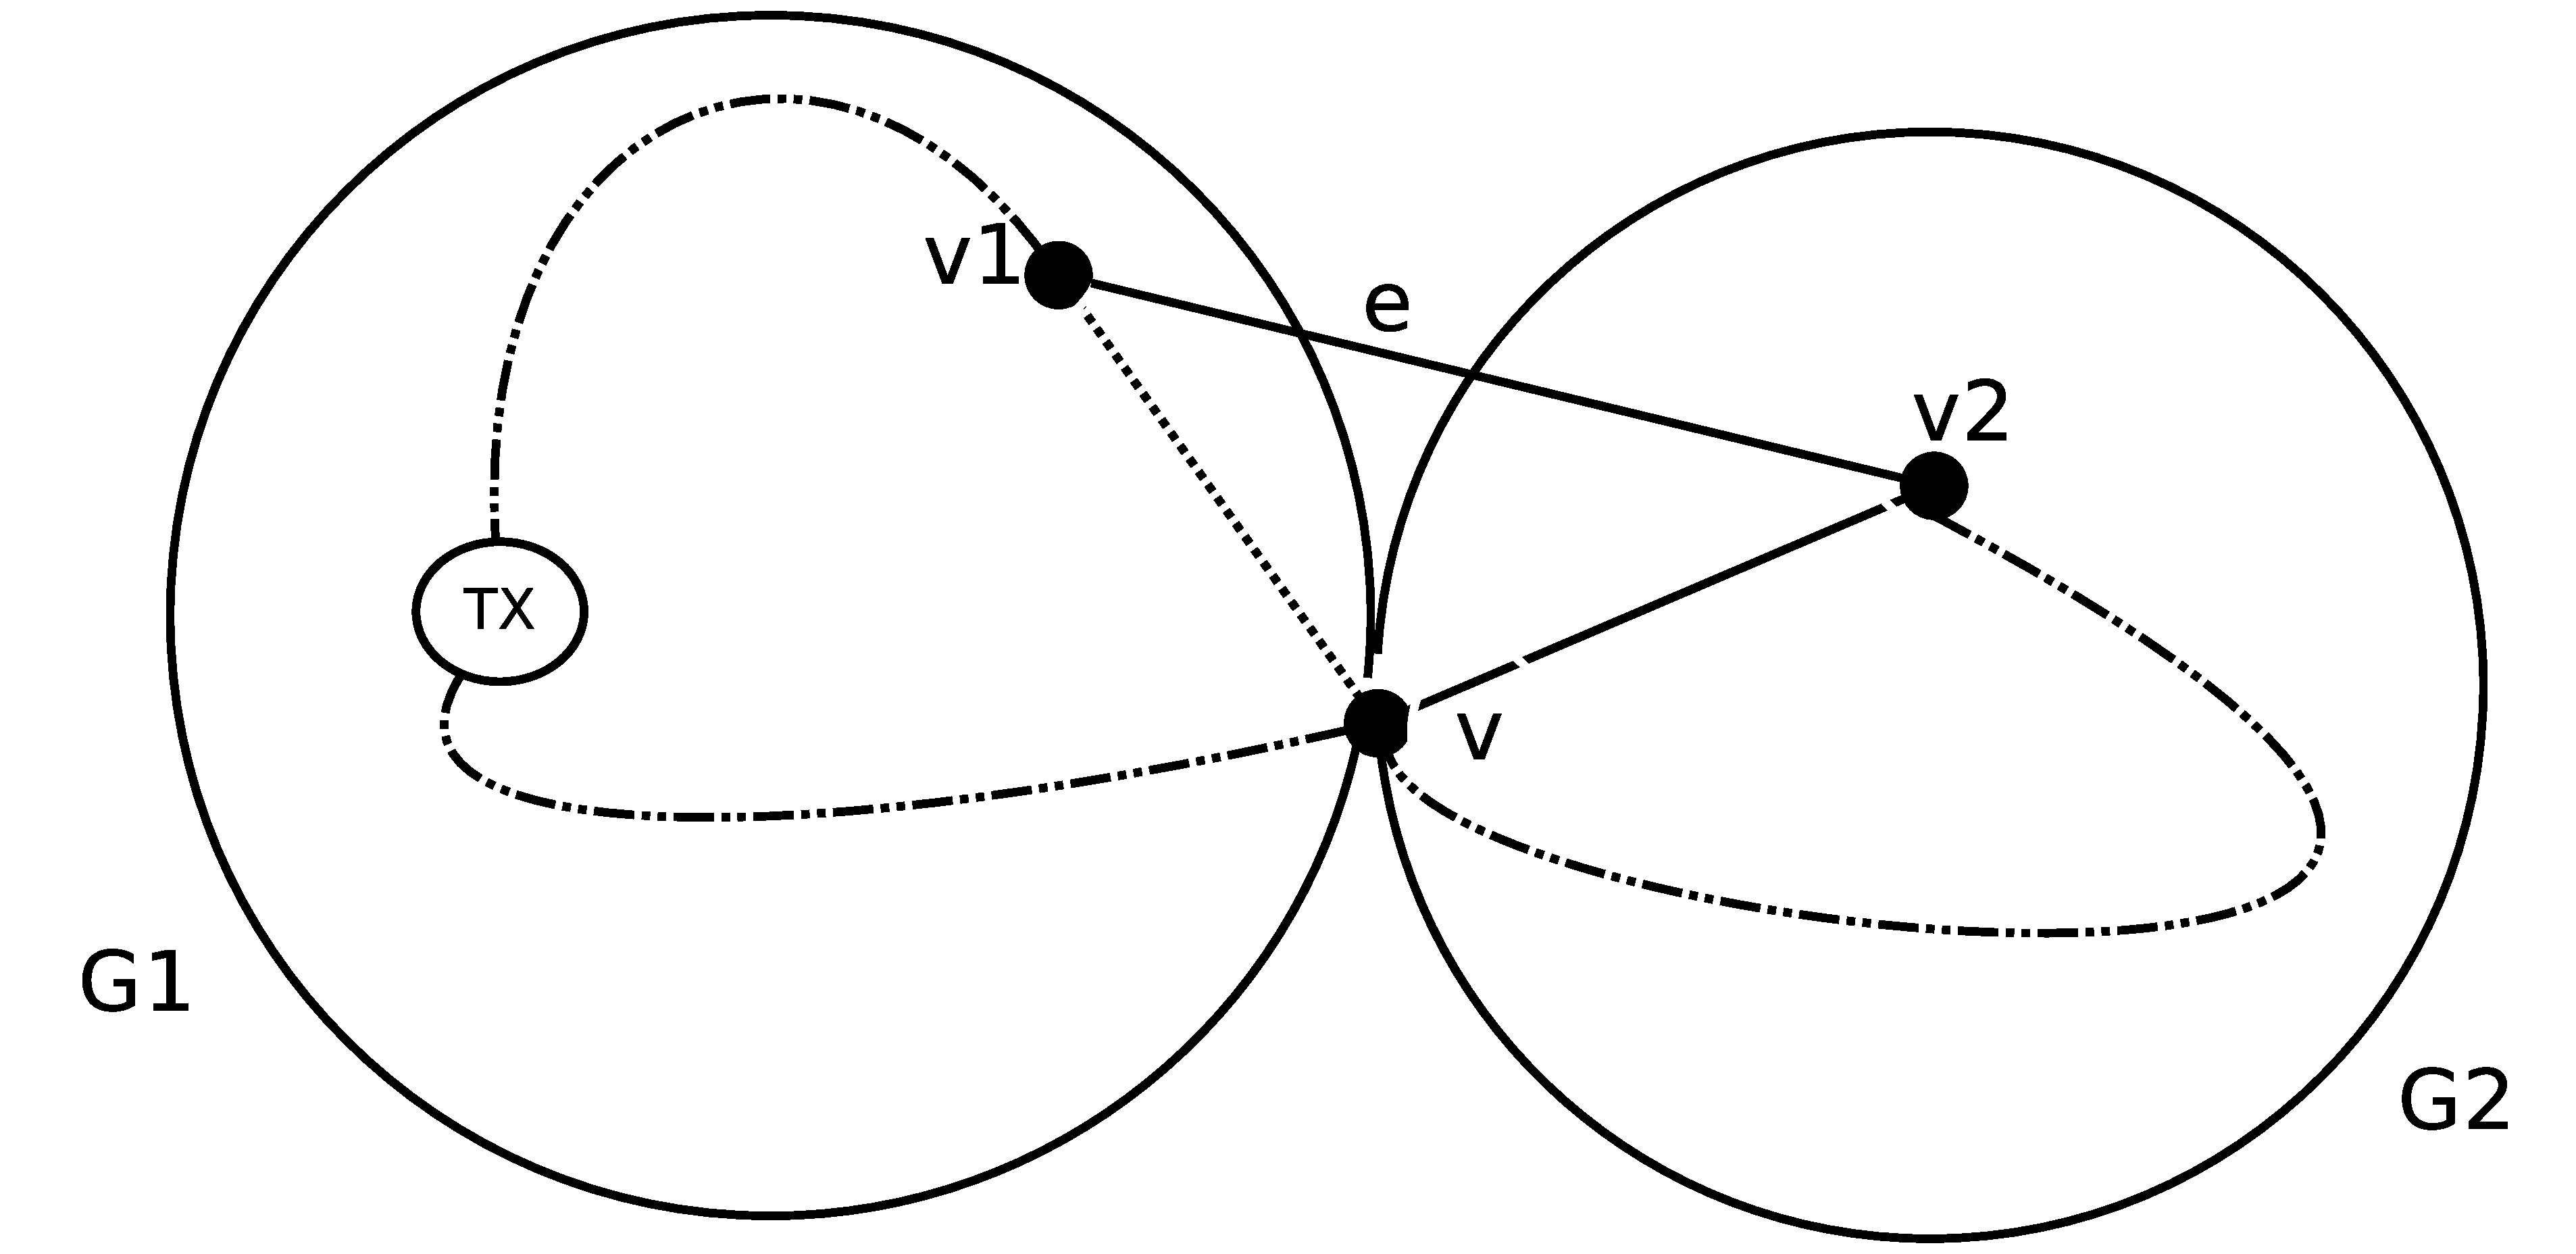
\includegraphics[height=2in]{figLemma4.4.4.eps} \\ 
	\caption{Lemma \ref{lemma4.4.4}: The graph $G$ consists of connected components $G_1$ and $G_2$, which are connected via vertex $v$ which is common to both components. If $G+e$ contains a $TX$, the so does either $G_1$ or $G_2$.}
\label{figLemma4.4.4}
\end{figure}

\begin{lemma}\label{lemma4.4.5}
If $|G| \geq 4|$ and $G$ is edge-maximal with $TK_5, TK_{3,3} \not\subseteq G$, then $G$ is 3-connected.
\end{lemma}
\begin{proof}
We apply induction on $|G|$. For $|G|=4$, the edge-maximal graph is $G=K_4$, which does not contain a $TK_5$ or $TK_{3,3}$, so $G=K_4$ is 3-connected. Now, consider the graphs for which $|G|>4$ such that $G$ is edge-maximal and does not contain a $TK_5$ or a $TK_{3,3}$. Suppose that $G$ has 2 connected components, $G_1$ and $G_2$, as in Lemma \ref{lemma4.4.4}. For the set of 3-connected graphs $\chi:=\{K_5, K_{3,3}\}$, Lemma \ref{lemma4.4.4} says that $G_1 \cap G_2$ is a $K_2$. Let $G_1 \cap G_2$ will be an edge connecting vertices $x$ and $y$. Also let $G_1$ and $G_2$ be edge-maximal and assume neither of them contain a $TK_5$ or $TK_{3,3}$. If that is the case, then $G_1$ and $G_2$ are either 3-connected or are triangles. Since $G_1$ and $G_2$ cannot contain $K_5$ or $K_{3,3}$ as minors, they are thus planar by lemma \ref{planar}. 

We can draw $G_1$ and $G_2$ as shown in Figure \ref{figLemma4.4.5}. Let $z_1$ and $z_2$ be two vertices in the boundaries of $G_1$ and $G_2$ respectively and let $K$ be a $TK_5$ or $TK_{3,3}$ in the graph $G+z_1 z_2$. If all of the branch vertices of $K$ lie in $G_1$ or in $G_2$, then either $G_i + xz_i$ or $G_i + yz_i$, for $i=1,2$, contains a $TK_5$ or $TK_{3,3}$. However, since $G_1$ and $G_2$ are planar, this contradicts Corollary \ref{corollary-euler}. 

What if the branch vertices are not all in either $G_1$ or $G_2$? Say the subgraphs $G_1$ and $G_2$ cannot both contain a branch vertex of a $TK_5$ because because $G+z_1 z_2$ does not contain four independent paths between $(G_1 - G_2)$ and $(G_2 - G_1)$. For the same reason, $G_1$ and $G_2$ cannot both contain two branch vertice of a $TK_{3,3}$. Then $K$ would be a $TK_{3,3}$ with only one branch vertex $v$ in $G_2 - G_1$ or $G_1 - G_2$. Let's say that $K$ is a $TK_{3,3}$ with only one branch vertex $v$ in $G_2 - G_1$. If this were the case then the graph $G_1 + v + \{vx,vy,vz_1\}$ , which is planar, contains a $TK_{3,3}$ We have a contradiction again of Corollary \ref{corollary-euler}.


\end{proof}
\begin{figure}[htbp]
	\centering
	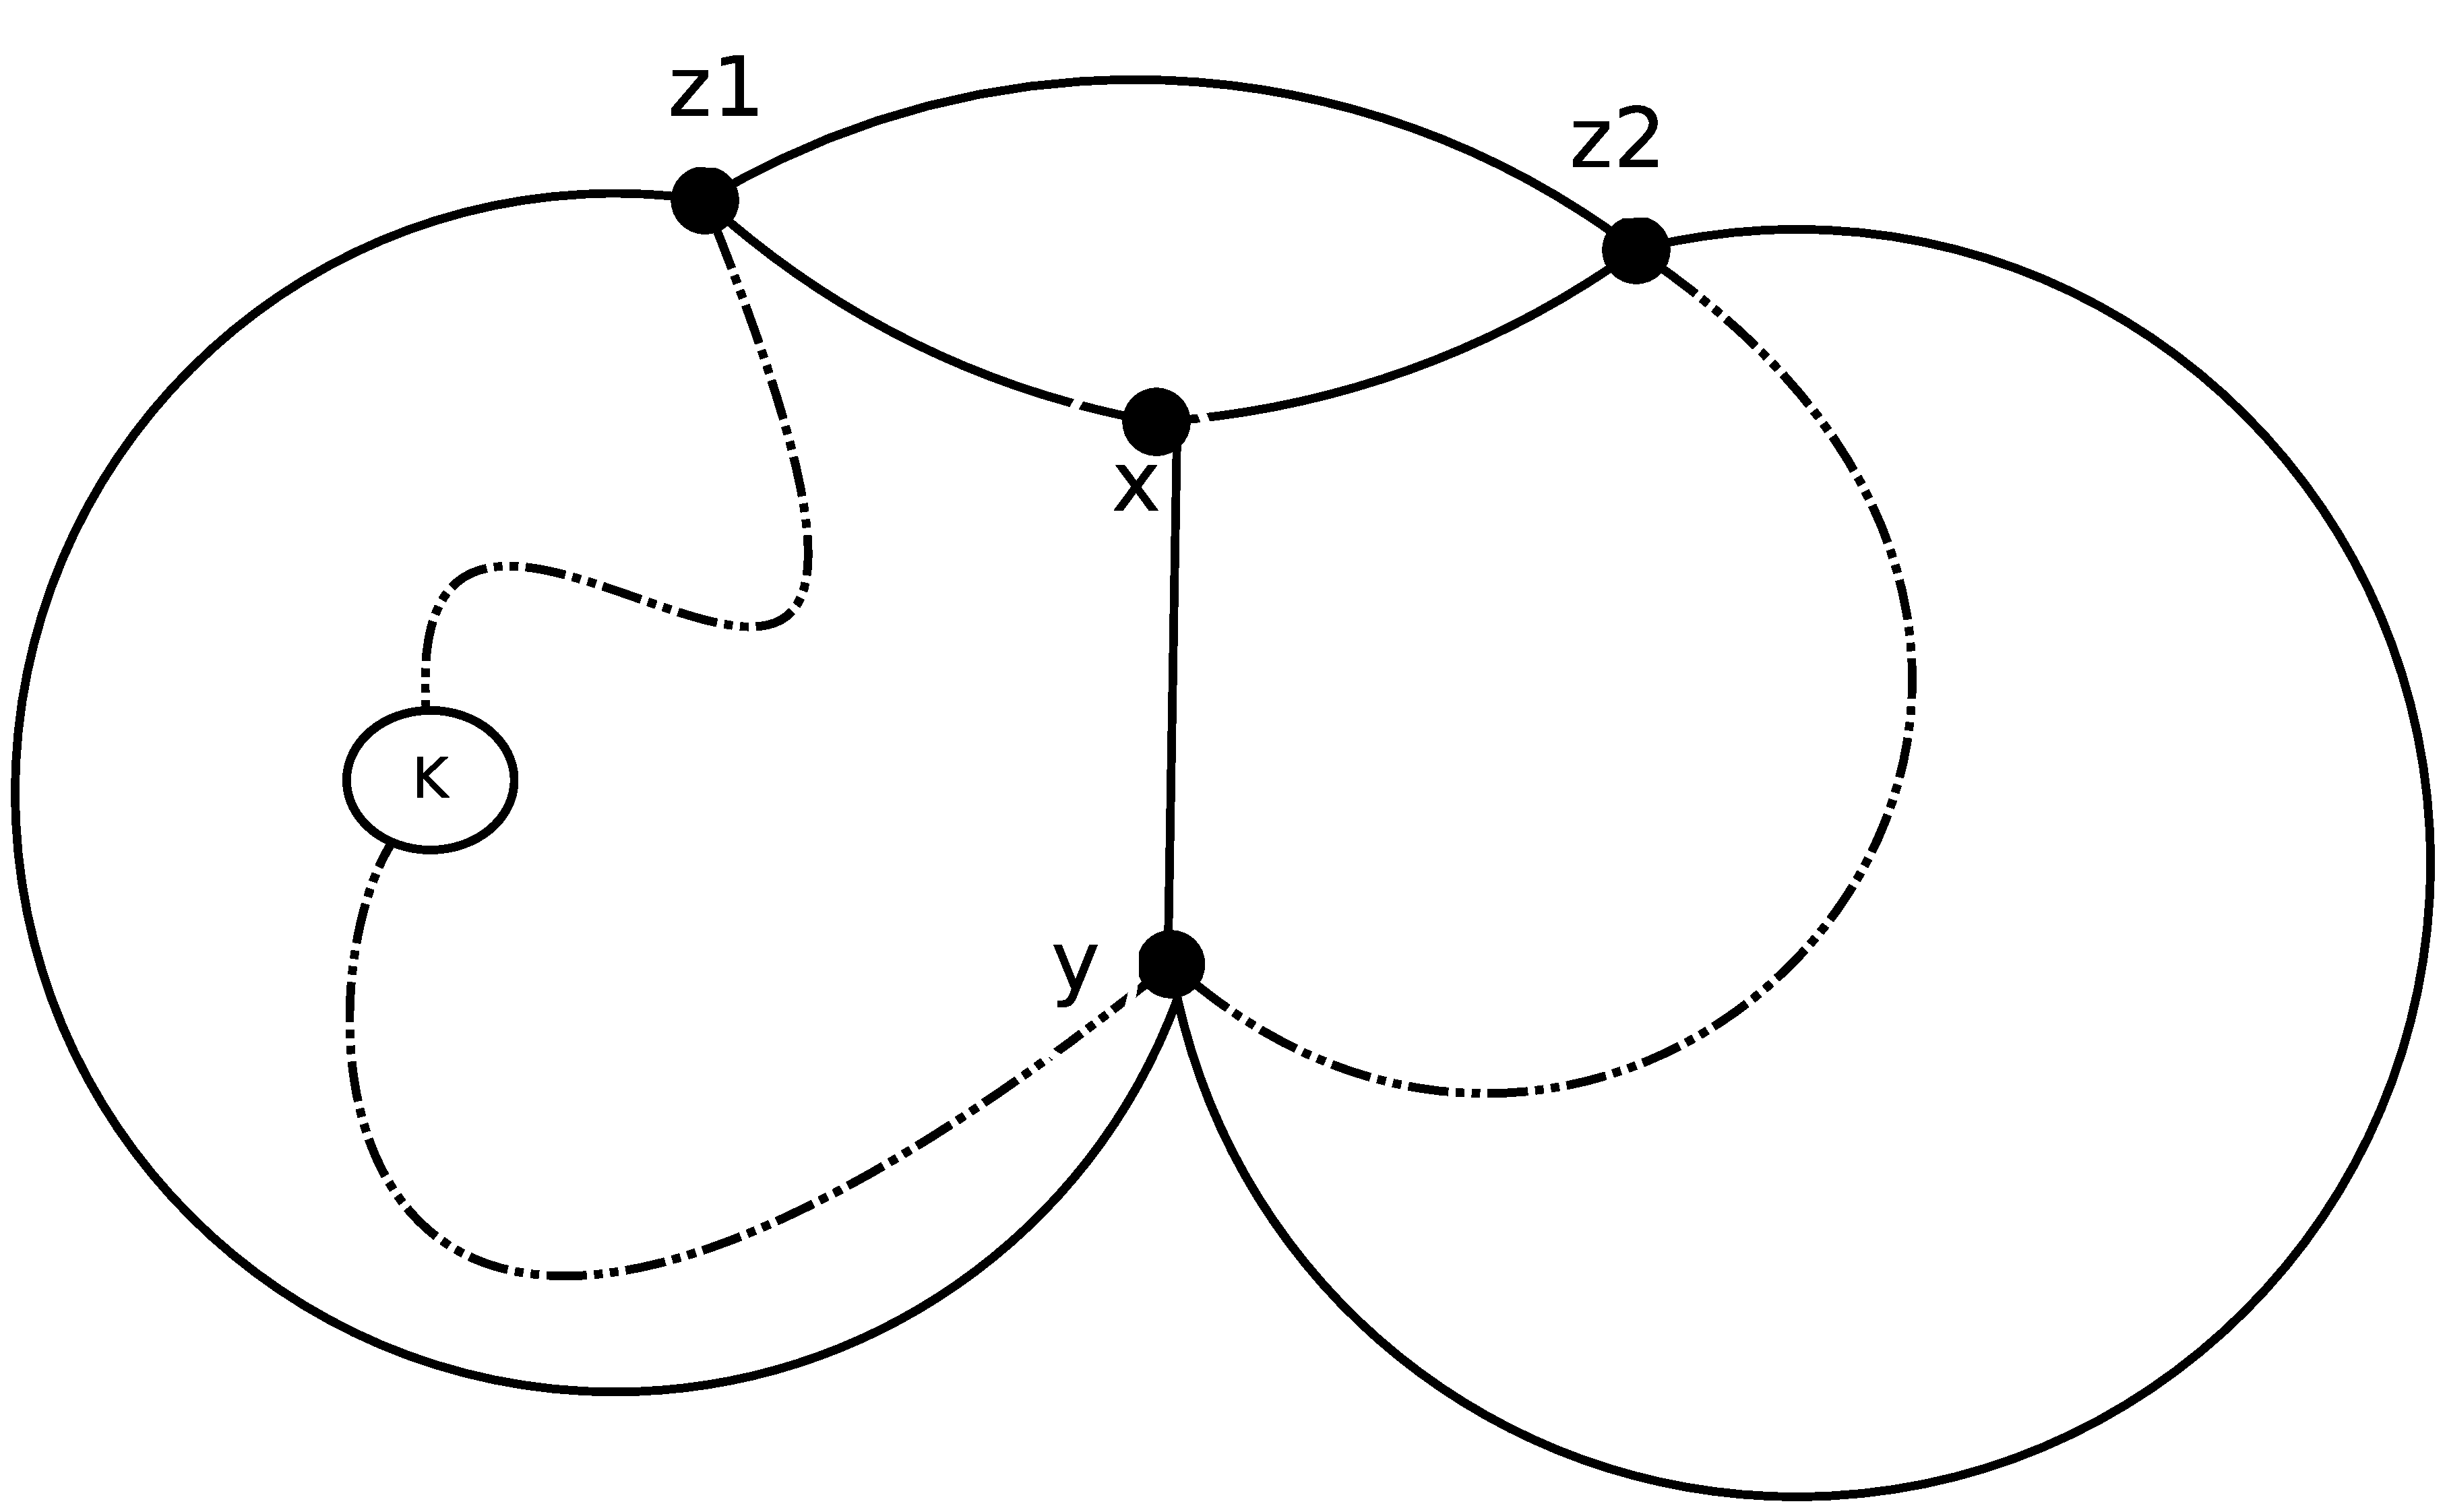
\includegraphics[height=2in]{figLemma4.4.5.eps} \\ 
	\caption{Lemma \ref{lemma4.4.5}: A $TK_5$ or $TK_{3,3}$ in $G + z_1 z_2$.}
\label{figLemma4.4.5}
\end{figure}


\subsection{Proof of Kuratowski's Theorem}

\begin{proof}
$(i) \Rightarrow (ii)$: Let G be a planar graph. Assume that there exists a $TK_5$ or $TK_{3,3}$ in $G$. Graphs $K_5$ and $K_{3,3}$ are not planar. By lemma \ref{lemma4.4.5}, $TK_5$ and $TK_{3,3}$ are not planar eit her. Since each subgraph of a planar graph needs to be planar, we have a contradiction.

$(ii) \Rightarrow (i)$: Let G be a graph that does not contain a $TK_5$ or a $TK_{3,3}$. We can add as many edges to G such that we do not create $TK_5$ or a $TK_{3,3}$. Then, by Lemma \ref{lemma4.4.5}, the resulting graph, $G'$, will be 3-connected. By Lemma \ref{minor_topoMinor} and Lemma \ref{lemma3.2.4} , since $G'$ is 3-connected and does not contain a $MK_5$ or $MK_{3,3}$, then $G'$ is planar. Since $G'$ is a minor of $G$, then $G$ is planar as well.

$(ii) \Rightarrow (iii)$: by Lemma \ref{minor_topoMinor}.

\end{proof}


\section{Conclusion}
We have proved using Kuratowski's Theorem that a graph is planar if the graph does not contain a minor of the graph $K_5$ or $K_{3,3}$.






